% main.tex - Hauptdatei der Vorlage
% Vorlage
%! LaTeX Vorlage
\documentclass[12pt, fleqn, captions=nooneline, titlepage, footsepline, headsepline, toc=chapterentrywithdots, listof=entryprefix, bibliography=totoc, parskip=half-]{scrreprt}

\usepackage{silence} %unnötige Warnungen unterdrücken
\WarningFilter{latex}{You have requested}
% \WarningFilter{scrlayer-scrpage}{\headheight to low}
% \WarningFilter{scrlayer-scrpage}{\footheight to low}
% \WarningFilter{scrlayer-scrpage}{Very small head height detected}
% \WarningFilter{fvextra}{} % was caused by loading csquotes before minted (which loads fvextra)
% \WarningFilter{lineno}{}

\pdfsuppresswarningpagegroup=1

\ProvidesPackage{metadaten}
\usepackage{metadaten}

\usepackage{tocbasic}
\usepackage[ngerman]{babel}
\usepackage[%
  backend=biber,
  labeldateparts=true,
  style=authortitle,
  isbn=false,
  dashed=false,
  maxnames=3]{biblatex}

%!  Änderungen für scrreprt
\renewcommand{\autodot}{}
\usepackage{chngcntr}
\counterwithout{figure}{chapter}
\counterwithout{table}{chapter}
\counterwithout{footnote}{chapter}
\RedeclareSectionCommand[style=section,afterskip=.15em]{chapter}
\setcounter{secnumdepth}{\subsubsectionnumdepth}
\setcounter{tocdepth}{\subsubsectionnumdepth}
\addtokomafont{chapter}{\LARGE}
\addtokomafont{section}{\Large}
\addtokomafont{subsection}{\large}
\addtokomafont{subsubsection}{\normalsize}
\renewcommand*{\chaptermarkformat}{}

%! Formatierung aller Verzeichnisse
%! Das Inhaltsverzeichnis wird an dieser Stelle formatiert.
\RedeclareSectionCommands[beforeskip=-.1\baselineskip, afterskip=.1\baselineskip, tocindent=0pt, tocnumwidth=45pt]{chapter, section,subsection,subsubsection}

\renewcaptionname{ngerman}{\refname}{Quellenverzeichnis}
\setuptoc{toc}{totoc}
\setuptoc{lof}{totoc}
\setuptoc{lot}{totoc}
\renewcommand*\listoflofentryname{\bfseries\figurename}
\BeforeStartingTOC[lof]{\renewcommand*\autodot{\space\space\space\space}}
\addtokomafont{captionlabel}{\bfseries}
\renewcommand*\listoflotentryname{\bfseries\tablename}
\BeforeStartingTOC[lot]{\renewcommand*\autodot{\space\space\space\space}}

%! Anhangsverzeichnis
\providecaptionname{ngerman}{\listofatocentryname}{Anhang}

\makeatletter
\AfterTOCHead[atoc]{\let\if@dynlist\if@tocleft}
\newcommand*{\useappendixtocs}{
  \renewcommand*{\ext@toc}{atoc}
  \RedeclareSectionCommands[tocindent=0pt]{chapter, section, subsection, subsubsection}
  \RedeclareSectionCommands[tocnumwidth=85pt]{chapter, section, subsection, subsubsection}
  \renewcommand*\listoflofentryname{\mdseries}
  \renewcommand{\thechapter}{\arabic{chapter}}
  \renewcommand{\@dotsep}{10000}
  }
\newcommand*{\usestandardtocs}{
  \renewcommand*{\ext@toc}{toc}
  }
\makeatother

%! Formelverzeichnis
\DeclareNewTOC[
  type=formel,                         % Name der Umgebung
  types=formeln,                       % Erweiterung (\listofschemes)
  float,                               % soll gleiten
  tocentryentrynumberformat=\bfseries, % voreingestellte Gleitparameter
  name=Formel,                         % Name in Überschriften
  listname={Formelverzeichnis},        % Listenname
  % counterwithin=chapter
]{lom}
\setuptoc{lom}{totoc}
\renewcommand*{\formelformat}{\hfill%
  \formelname~\theformel%
  \autodot{\space\space\space}
}
\BeforeStartingTOC[lom]{\renewcommand*\autodot{\space\space\space\space}}

%! Inhalts-/Anhangsverzeichnis
\DeclareNewTOC[%
  %owner=\jobname,
  tocentrystyle=tocline,
  tocentryentrynumberformat=\PrefixBy{Anhang},
  listname={Anhangsverzeichnis}% Titel des Verzeichnisses
]{atoc}% Dateierweiterung (a=appendix, toc=table of contents)

\usepackage{xpatch}
\xapptocmd\appendix{%
  \useappendixtocs
  \listofatocs
  \addcontentsline{toc}{chapter}{Anhangsverzeichnis}
  \newpage
  \pagenumbering{gobble}
  \pagestyle{scrheadings}
  \clearmainofpairofpagestyles
  \clearplainofpairofpagestyles
  \rohead{\textnormal{Anhang~\arabic{chapter}}}
  \lohead{\textnormal{\currentname}}
  \lofoot{}
  \cofoot{}
  \rofoot{}
}{}{}

\DeclareNewTOC[
  type=example,                         % Name der Umgebung
  types=examples,                       % Erweiterung (\listofschemes)
  float,                               % soll gleiten
  tocentryentrynumberformat=\bfseries, % voreingestellte Gleitparameter
  name=Beispiel,                         % Name in Überschriften
  listname={Beispielverzeichnis},        % Listenname
  % counterwithin=chapter
]{lob}
\setuptoc{lob}{totoc}


%! Ermöglicht die Ausgabe des aktuellen Titels.
\usepackage{nameref}
\makeatletter
\newcommand*{\currentname}{\@currentlabelname}
\makeatother

%! zusätzliche LaTeX-Packages
\usepackage{amsmath}
\usepackage{amssymb}
\usepackage{amsthm}
\usepackage{tabularx}
\usepackage{multirow}
\usepackage{setspace}
\usepackage{booktabs}
\usepackage{svg}
\usepackage{graphicx}
\usepackage{float}
\usepackage[a4paper,lmargin={2.5cm},rmargin={2.5cm},tmargin={2cm},bmargin={2cm}]{geometry}
\usepackage{lineno}
\usepackage[T1]{fontenc}
\usepackage{listings}
\usepackage{tikz}
\usepackage{varwidth}
\usepackage{ifthen}
\usepackage{etoolbox}

%! Abbildungen von Verzeichnisstrukturen

\usepackage{dirtree}

%! Centered Dirtree - https://tex.stackexchange.com/posts/100182/revisions
\makeatletter
\def\dirtree#1{%
  %%2012\let
  \DT@indent=\parindent
  \parindent=\z@
  %%2012\let
  \DT@parskip=\parskip
  \parskip=\z@
  %%2012\let
  \DT@baselineskip=\baselineskip
  \baselineskip=\DTbaselineskip
  \let\DT@strut=\strut
  \def\strut{\vrule width\z@ height0.7\baselineskip depth0.3\baselineskip}%
  \DT@counti=\z@
  \let\next\DT@readarg
  \next#1\@nil
  \dimen\z@=\hsize
  \advance\dimen\z@ -\DT@offset
  \advance\dimen\z@ -\DT@width
%  \setbox\z@=\hbox to\dimen\z@{%
  \setbox\z@=\hbox{%
%    \hsize=\dimen\z@
    \vbox{\hbox{\@nameuse{DT@body@1}}}%
  }%
  \dimen\z@=\ht\z@
  \advance\dimen0 by\dp\z@
  \advance\dimen0 by-0.7\baselineskip
  \ht\z@=0.7\baselineskip
  \dp\z@=\dimen\z@
  \par\leavevmode
  \kern\DT@offset
  \kern\DT@width
  \box\z@
  \endgraf
  \DT@countii=\@ne
  \DT@countiii=\z@
  \dimen3=\dimen\z@
  \@namedef{DT@lastlevel@1}{-0.7\baselineskip}%
  \loop
  \ifnum\DT@countii<\DT@counti
    \advance\DT@countii \@ne
    \advance\DT@countiii \@ne
    \dimen\z@=\@nameuse{DT@level@\the\DT@countii}\DT@all
    \advance\dimen\z@ by\DT@offset
    \advance\dimen\z@ by-\DT@all
    \leavevmode
    \kern\dimen\z@
    \DT@countiv=\DT@countii
    \count@=\z@
    %%2012\LOOP
    \DT@loop
      \advance\DT@countiv \m@ne
      \ifnum\@nameuse{DT@level@\the\DT@countiv} >
        \@nameuse{DT@level@\the\DT@countii}\relax
      \else
        \count@=\@ne
      \fi
    \ifnum\count@=\z@
    %%2012\REPEAT
    \DT@repeat
    \edef\DT@hsize{\the\hsize}%
    \count@=\@nameuse{DT@level@\the\DT@countii}\relax
    \dimen\z@=\count@\DT@all
    \advance\hsize by-\dimen\z@
    \setbox\z@=\vbox{\hbox{\@nameuse{DT@body@\the\DT@countii}}}%
    \hsize=\DT@hsize
    \dimen\z@=\ht\z@
    \advance\dimen\z@ by\dp\z@
    \advance\dimen\z@ by-0.7\baselineskip
    \ht\z@=0.7\baselineskip
    \dp\z@=\dimen\z@
    \@nameedef{DT@lastlevel@\the\DT@countii}{\the\dimen3}%
    \advance\dimen3 by\dimen\z@
    \advance\dimen3 by0.7\baselineskip
    \dimen\z@=\@nameuse{DT@lastlevel@\the\DT@countii}\relax
    \advance\dimen\z@ by-\@nameuse{DT@lastlevel@\the\DT@countiv}\relax
    \advance\dimen\z@ by0.3\baselineskip
    \ifnum\@nameuse{DT@level@\the\DT@countiv} <
        \@nameuse{DT@level@\the\DT@countii}\relax
      \advance\dimen\z@ by-0.5\baselineskip
    \fi
    \kern-0.5\DT@rulewidth
    \hbox{\vbox to\z@{\vss\hrule width\DT@rulewidth height\dimen\z@}}%
    \kern-0.5\DT@rulewidth
    \kern-0.5\DT@dotwidth
    \vrule width\DT@dotwidth height0.5\DT@dotwidth depth0.5\DT@dotwidth
    \kern-0.5\DT@dotwidth
    \vrule width\DT@width height0.5\DT@rulewidth depth0.5\DT@rulewidth
    \kern\DT@sep
    \hbox{\box\z@}%
    \endgraf
  \repeat
  \parindent=\DT@indent
  \parskip=\DT@parskip
  %%2012\DT@baselineskip=\baselineskip
  \baselineskip=\DT@baselineskip
  \let\strut\DT@strut
}

\makeatother


%! PageBreaks nach jeder Section
\let\oldchapter\chapter
\renewcommand\chapter{\clearpage\oldchapter}

%! Code-Umgebungen
%! Code-Integration im Dokument
%? Inklusive Erzeugung eines Custom-Enviroments für Programmcodes
\usepackage{minted}

% ! Anpassung der Minted-Umgebung, um Abstände zu vereinheitlichen und die Optik zu verbessern
\let\oldminted\minted
\let\oldendminted\endminted
\def\minted{\begingroup \vspace{-0.3cm} \oldminted}
\def\endminted{\oldendminted \vspace{-0.5cm} \endgroup}

\xapptocmd{\inputminted}{\vspace{-0.5cm}}{}{}

%Zeilennummern neu definieren, um Warnungen zu vermeiden und modern anmutende Zahlen zu nutzen
\renewcommand{\theFancyVerbLine}{\scriptsize{\arabic{FancyVerbLine}}}

%Standardformatierung für minted-Umgebung erstellen
\setminted{
    tabsize=2,
    breaklines,
    autogobble,
    fontfamily=courier,
    linenos,
    %! see https://pygments.org/demo/#try, other nice options: paraiso-light, solarized-light, rainbow_dash, gruvbox-light, stata, tango
    style=emacs
}
%Keine Zeilennnummer, wenn der einzeilige \mint-Befehl genutzt wird
\xpretocmd{\mint}{\setminted{linenos=false}}{}{}
\xpretocmd{\minted}{\setminted{linenos=true}}{}{}

\DeclareNewTOC[
  type=code,                           % Name der Umgebung
  types=codes,                         % Erweiterung (\listofschemes)
  float,                               % soll gleiten
  floatpos=h,
  tocentryentrynumberformat=\bfseries, % voreingestellte Gleitparameter
  name=Code,                           % Name in Überschriften
  listname={Programmcodeverzeichnis},  % Listenname
  % counterwithin=chapter
]{loc}
\setuptoc{loc}{totoc}

\renewcommand*{\codeformat}{%
  \codename~\thecode%
  \autodot{\space\space\space}
}
\BeforeStartingTOC[loc]{\renewcommand*\autodot{\space\space\space\space}}
\AtBeginEnvironment{minted}{\vspace{\baselineskip}}


\usepackage{scrhack} %necessary to use float with scrreprt
\usepackage{csquotes}

%! Schriftart
%! Die HAWA schreibt Arial vor, welches in Standard LaTeX-Distributionen nicht mitgeliefert wird. Helvetica ist nahezu identisch.
\usepackage{helvet}
\usepackage{microtype}
\renewcommand{\familydefault}{\sfdefault}
%! Hyperref und PDF-meta
\usepackage[hidelinks]{hyperref}

%! PDF-Metadaten (Autor/Titel/Beschreibung)
%! PDF-Metadaten
\hypersetup{pdftitle={\titel}}
\hypersetup{pdfsubject={\kurzbeschreibung}}
\ifthenelse{\isundefined{\autorzwei}}{\hypersetup{pdfauthor={\autoreins}}}{%
    \ifthenelse{\isundefined{\autordrei}}{\hypersetup{pdfauthor={\autoreins, \autorzwei}}}{%
        \ifthenelse{\isundefined{\autorvier}}{\hypersetup{pdfauthor={\autoreins, \autorzwei, \autordrei}}}{%
        \hypersetup{pdfauthor={\autoreins, \autorzwei, \autordrei, \autorvier}}
        }
    }
}

\usepackage[numbered]{bookmark}
\usepackage[printonlyused]{acronym}
\usepackage{enumitem}

%Abkürzungsverzeichnis - Formatierung (bspw. zur korrekten Anzeige von BASH-Befehlen)
\renewcommand*{\aclabelfont}[1]{\acsfont{#1}}

%! Untertitel/Legenden
\usepackage{caption}
% Captions linksbündig, auch wenn einzeilig
\captionsetup{
  labelsep=none,
  justification=raggedright,
  singlelinecheck=false
}
\renewcommand*{\figureformat}{%
  \figurename~\thefigure%
  \autodot{\space\space\space}
}
\renewcommand*{\tableformat}{%
  \tablename~\thetable%
  \autodot{\space\space\space}
}


%! Literaturverzeichnis und Zitierbefehle
%! Formatierung des Literaturverzeichnis
\DeclareLabeldate{%
\field{year}
}

\DeclareExtradate{%
\scope{
\field{labelyear}
\field{year}}
}
\DeclareFieldFormat{url}{In: \url{#1}}
\DeclareFieldFormat{urldate}{\space\mkbibparens{#1}}
\DeclareFieldFormat{urlday}{\forcezerosmdt{#1}}
\DeclareFieldFormat{urlmonth}{\forcezerosmdt{#1}}
\DeclareFieldFormat{urlyear}{\forcezerosmdt{#1}}
\DeclareFieldFormat{date}{#1\printfield{extradate}}

\urlstyle{same}
%? Author-Format für Literaturverzeichnis
\DeclareNameFormat{author}{%
  \nameparts{#1}%
  \usebibmacro{name:family-given}
    {\expandafter\ifblank\expandafter{\namepartgiven}
       {\namepartfamily}% no family name, don't uppercase
       {\MakeUppercase{\namepartfamily}}%
    }
    {\namepartgiven}
    {\namepartprefix}
    {\namepartsuffix}%
    \ifthenelse{\value{listcount}=1\AND\ifmorenames}{\andothersdelim\bibstring{andothers}}{}%
}
%? Author-Format für Fußnoten
\DeclareNameFormat{author_fn}{%
\nameparts{#1}%
\usebibmacro{name:family}
  {\expandafter\ifblank\expandafter{\namepartgiven}
     {\namepartfamily}% no family name, don't uppercase
     {\MakeUppercase{\namepartfamily}}%
  }
  {\namepartgiven}
  {\namepartprefix}
  {\namepartsuffix}%
  \ifthenelse{\value{listcount}=1\AND\ifmorenames}{\andothersdelim\bibstring{andothers}}{}%
}
\DeclareFieldFormat{title}{#1}

\renewcommand{\multinamedelim}{\addsemicolon\space}
\renewcommand{\finalnamedelim}{\addsemicolon\space}
\renewcommand{\labelnamepunct}{\addcolon\space}
\renewcommand*{\finentrypunct}{}
\renewcommand{\andothersdelim}{\addsemicolon\space}

\setlength\bibitemsep{\baselineskip}
\setlength\bibhang{0pt}

%! Formatierung der Fußnotenzitate / Literaturverzeichnis
\renewcommand*{\newunitpunct}{\addcomma\space}

%? Normales Zitat...
\DeclareCiteCommand{\zitat}[\mkbibfootnote]
  {\usebibmacro{prenote}}
  {\usebibmacro{citeindex}
   \setunit{\addnbspace}
   \bibhyperref{\printnames[author_fn]{labelname}}
   \setunit{\labelnamepunct}
   \newunit
   \printfield{location}
   \newunit
   \printfield{labelyear}\printfield{extradate}
   \newunit
   \printfield{pages}
   }
  {\addsemicolon\space}
  {\usebibmacro{postnote}}

%? Online Zitat
\DeclareCiteCommand{\onlinezitat}[\mkbibfootnote]
  {\usebibmacro{prenote}}
  {\usebibmacro{citeindex}
   \setunit{\addnbspace}
   online:
   \bibhyperref{\printnames[author_fn]{labelname}}
   \setunit{\labelnamepunct}
   \newunit
   \printfield{labelyear}\printfield{extradate}
   \printtext{(}\printfield{urlday}\printtext{.}\printfield{urlmonth}\printtext{.}\printfield{urlyear}\printtext{)}}
  {\addsemicolon\space}
  {\usebibmacro{postnote}}

%? Sinngemäßes Zitat
\DeclareCiteCommand{\vgzitat}[\mkbibfootnote]
  {\usebibmacro{prenote}}
  {\usebibmacro{citeindex}
   \setunit{\addnbspace}
   vgl. 
   \bibhyperref{\printnames[author_fn]{labelname}}
   \setunit{\labelnamepunct}
   \newunit
   \printfield{location}
   \newunit
   \printfield{labelyear}\printfield{extradate}
   \newunit
   \printfield{pages}
   }
  {\addsemicolon\space}
  {\usebibmacro{postnote}}


%? Sinngemäßes Online Zitat
\DeclareCiteCommand{\vgonlinezitat}[\mkbibfootnote]
  {\usebibmacro{prenote}}
  {\usebibmacro{citeindex}
   \setunit{\addnbspace}
   vgl. online:
   \bibhyperref{\printnames[author_fn]{labelname}}
   \setunit{\labelnamepunct}
   \newunit
   \printfield{labelyear}\printfield{extradate}
   \printtext{(}\printfield{urlday}\printtext{.}\printfield{urlmonth}\printtext{.}\printfield{urlyear}\printtext{)}}
  {\addsemicolon\space}
  {\usebibmacro{postnote}}

%? Unveröffentlichtes Zitat
\DeclareCiteCommand{\uvzitat}[\mkbibfootnote]
  {\usebibmacro{prenote}}
  {\usebibmacro{citeindex}
   \setunit{\addnbspace}
   unveröffentlicht:
   \bibhyperref{\printnames[author_fn]{labelname}}
   \setunit{\labelnamepunct}
   \newunit
   \printfield{location}
   \newunit
   \printfield{labelyear}\printfield{extradate}
   \newunit
   \printfield{pages}
   }
  {\addsemicolon\space}
  {\usebibmacro{postnote}}

%? Sinngemäßes, unveröffentlichtes Zitat
\DeclareCiteCommand{\vguvzitat}[\mkbibfootnote]
{\usebibmacro{prenote}}
{\usebibmacro{citeindex}
 \setunit{\addnbspace}
 vgl. unveröffentlicht:
 \bibhyperref{\printnames[author_fn]{labelname}}
 \setunit{\labelnamepunct}
 \newunit
 \printfield{location}
 \newunit
 \printfield{labelyear}\printfield{extradate}
 \newunit
 \printfield{pages}
 }
{\addsemicolon\space}
{\usebibmacro{postnote}}



\renewcommand{\bibfootnotewrapper}[1]{\bibsentence#1}

\DeclareMultiCiteCommand{\zitate}[\mkbibfootnote]{\footpartcite}{\addsemicolon\space}
\addbibresource{literatur.bib}



%! Kopf- und Fußzeilen
\input{vorlage/vorlage_subs/kopf_fußzeile}

%! verbesserte Umbrüche (hoffentlich)
\input{vorlage/vorlage_subs/umbrüche}

% vordefinierte Kommandos der Vorlage
%! Eigene Befehle zur erleichterten Nutzung
% Hilfsbefehle
\newcommand{\fontheightsvg}[1]{\includesvg[height=1.75ex, inkscapelatex=false]{#1}}
\newcommand{\dtfolder}{\fontheightsvg{vorlage/bilder/dirtree_folder}\hspace{0.1cm}}
\newcommand{\dtfile}{\fontheightsvg{vorlage/bilder/dirtree_file}\hspace{0.1cm}}

% Umgebungen u.Ä.
\newcommand{\fn}[1]{\footnote{\hspace{0.5em}#1}}
%! #1 - Breite, #2 - Dateiname, #3 Caption, #4 - Label
\newcommand{\bild}[4][1.0]{\begin{figure}[hptb]
  \centering
  \includegraphics[width=#1\columnwidth]{bilder/#2}
  \caption{#3}
  \label{#4}
  \end{figure}}
\newcommand{\striche}[1]{\glqq #1\grqq{}}
%! #1 - Breite, #2 - Dateiname, #3 Caption, #4 - Label
\newcommand{\svg}[4][1.0]{\begin{figure}[hptb]
    \centering
    \includesvg[width=#1\columnwidth,inkscapelatex=false]{bilder/#2}
    \caption{#3}
    \label{#4}
    \end{figure}}
%! #1 - Dirtree, #2 - Caption, #3 - Label
\newcommand{\verzeichnis}[3]{\begin{figure}[H]
  % https://tex.stackexchange.com/a/99591/220899
  \renewcommand{\DTstyle}{\textrm\expandafter\raisebox{-0.7ex}}
  \centering
  \begin{varwidth}{\textwidth}
    \dirtree{#1}  
  \end{varwidth}
  \caption{#2}
  \label{#3}
  \end{figure}}
\newcommand{\logisch}[1]{$``#1``$}
\newcommand{\vglink}[2]{\fn{vgl.~\href{#1}{#1}~(#2)}}
% Muss statt \caption in die Umgebung wenn eine Fußnote verwendet werden soll, in Verbindung mit der Zeile darunter
\newcommand{\linkcaption}[1]{\caption[#1]{#1\footnotemark}}
% Muss unter die Umgebung, wenn eine Fußnote in der Umgebung verwendet werden soll
\newcommand{\vgcaption}[2]{\footnotetext{\hspace{0.5em}vgl.~\href{#1}{#1}~(#2)}}
\newcommand{\python}[1]{\mintinline{python}{#1}}
%! #1 - Formel, #2 - Legende, #3 - Caption, #4 - Label
\newcommand{\formula}[4]{\begin{formel}[hptb]
  \pretocmd{\captionbelow}{\onelinecaptionstrue}{}{}
  \KOMAoptions{captions=centeredbeside}
  \begin{captionbeside}[#3]{\textbf{#3}}[r]#1\end{captionbeside}
  \pretocmd{\captionbelow}{}{}{}#2\label{#4}\end{formel}}

% Referenzierung
\newcommand{\uniliteref}[2]{\emph{\hyperref[{#2}]{#1 \ref{#2} - \nameref{#2}}}}
\newcommand{\unifullref}[2]{(\emph{\hyperref[{#2}]{siehe #1 \ref{#2} - \nameref{#2}}})}

% Anhänge - Sonderbehandlung, da nameref auf Anhänge nicht funktioniert
% https://github.com/DSczyrba/Vorlage-Latex/issues/29
\newcommand{\litearef}[1]{\uniliteref{Anhang}{#1}}
\newcommand{\fullaref}[1]{\unifullref{Anhang}{#1}}
\newcommand{\aref}[1]{\litearef{#1}}
% Abbildungen
\newcommand{\litebref}[1]{\uniliteref{Abbildung}{#1}}
\newcommand{\fullbref}[1]{\unifullref{Abbildung}{#1}}
\newcommand{\bref}[1]{\litebref{#1}}
% Code
\newcommand{\litecref}[1]{\uniliteref{Code}{#1}}
\newcommand{\fullcref}[1]{\unifullref{Code}{#1}}
\newcommand{\cref}[1]{\litecref{#1}}
% Formeln
\newcommand{\litefref}[1]{\uniliteref{Formel}{#1}}
\newcommand{\fullfref}[1]{\unifullref{Formel}{#1}}
\newcommand{\fref}[1]{\litefref{#1}}
% Kapitel
\newcommand{\fullsref}[1]{\unifullref{Kapitel}{#1}}
\newcommand{\litesref}[1]{\uniliteref{Kapitel}{#1}}
\newcommand{\sref}[1]{\litesref{#1}}
% Tabellen
\newcommand{\litetref}[1]{\uniliteref{Tabelle}{#1}}
\newcommand{\fulltref}[1]{\unifullref{Tabelle}{#1}}
\newcommand{\tref}[1]{\litetref{#1}}
% Kompatibilität
\newcommand{\literef}[1]{\litesref{#1}}
\newcommand{\fullref}[1]{\fullsref{#1}}
% Auf gleiche Art können auch eigene Kommandos in eine Datei wie 'inhalt/kommandos.tex' ausgelagert werden

%Dokument-Anfang
\begin{document}

%! #########################################
%! Inhalt der Arbeit
\frontmatter

%Titelseite
\begin{titlepage}
    \begin{minipage}{0.7\columnwidth}
        \includesvg[width=\columnwidth]{vorlage/bilder/ba-gc-logo}
    \end{minipage}
    \begin{center}
        \Huge
        \vspace{.1\pdfpageheight}
        
        \textbf{Hinweise zur Anfertigung von wissenschaftlichen Arbeiten \vspace{.2\pdfpageheight}}
        
        \Large
        \textbf{Berufsakademie Sachsen\\Staatliche Studienakademie Glauchau}
        \normalsize
        \vfill
        \textbf{nach 4BA-F.207\\\vspace{1cm}Version 5.1}
    \end{center}
\end{titlepage}
\newpage
    
\lofoot{\textnormal{Version 5.1}}
%! Nicht benötigte Verzeichnisse hier auskommentieren
%? Inhaltsverzeichnis
\vfuzz=5pt
\tableofcontents
\newpage
\vfuzz=0.1pt

%? Abbildungsverzeichnis
\listoffigures
\newpage

%? Tabellenverzeichnis
\listoftables
\newpage

%? Formelverzeichnis
\listofformeln
\newpage

%? Abkürzungsverzeichnis
\include{inhalt/Abkürzungen}

%? Beispielverzeichnis
\listofexamples
\newpage

%? Begleitwort
\addchap{Begleitwort des Direktors}
Das Prinzip der Berufsakademie, Studierende dual an den beiden Lehr- und Lernorten – Staatliche Studienakademie und Praxispartner – auszubilden, bewährt sich seit der \ac{BA} im tertiären Bildungssektor. Wissenschaftliche Erkenntnisse und Methoden, die an beiden Orten zur Anwendung gelangen sowie Lösungsstrategien mit hohem praktischem Bezug, charakterisieren dieses duale Studium. Studienbegleitend ist eine Vielzahl von Dokumentationen (Projektarbeiten, Praxisarbeiten, Belege, Bachelorthesis, Diplomarbeit usw.) zu erstellen.

Die nachfolgende Anleitung soll Wegweiser und Hilfestellung sein, diese Ausarbeitungen nach aktuellen wissenschaftlichen Erkenntnissen und Methoden, sprachlich korrekt, formal exakt und innovativ zu verfassen.


%! Hier beginnt der eigentliche Inhalt der Arbeit.
\mainmatter

%! Eine der folgenden Zeilen wieder aktivieren und entsprechende Datei ablegen
%? druckt Firmenlogo ab Kapitel 1 in Kopfzeile - SVG ist, auch bei kleinen Grafiken, zu bevorzugen, wenn vorhanden
%\lohead{\includesvg[height=8mm,inkscapelatex=false]{bilder/firmenlogo}}
%\lohead{\includegraphics[height=8mm]{bilder/firmenlogo}}

% Es ist möglich, die ganze Arbeit in eine Datei (z.B. "Inhalt.tex") zu schreiben,
% allerdings empfiehlt es sich, zur besseren Strukturierung mehrere Dateien, bspw. eine pro Kapitel, zu verwenden.
% Diese werden folgendermaßen eingebunden:
%\include{inhalt/Inhalt}

%! Doku-/Testinhalt, diese Zeile bei Nutzung der Vorlage entfernen
\chapter{Zielsetzung}
\label{zielsetzung}
\section{Bemerkungen}
\label{zielsetzung-bemerkungen}
Eines der zu bewältigenden Probleme bei der Anfertigung von wissenschaftlichen Arbeiten hat seine Ursache in der herrschenden Datenflut.
Vom Verfasser wird eine systematische und akribische Vorgehensweise bei der Sichtung und Auswahl der Quellen verlangt.
Die wissenschaftlichen Bibliotheken bieten diverse Datenbanken, Kataloge
und andere elektronische Medien zur Unterstützung dieses Arbeitsprozesses an.
Für die Aufbereitung und Verwaltung der Quellen können Literaturverwaltungsprogramme genutzt werden.

Verwendet man das Internet als Quelle, sollte genau hinterfragt werden, ob es sich nicht um eine Fälschung oder ein Plagiat handelt.
Dem Verfasser bleibt es selbst überlassen, welche Qualitätsansprüche er an seine Arbeit stellt.
Eine Arbeit, die nur aus Internetquellen besteht, wird nie wissenschaftlichen Ansprüchen genügen. %TODO entfernen weil schwachsinn

Zur Überprüfung von wissenschaftlichen Arbeiten wird Software benutzt, die Plagiate erkennt.


\section{Projektarbeit}
\label{zielsetzung-projektarbeit}
In der Projektarbeit\fn{Projektarbeit wird als Synonym für Praxistransferbeleg, Praxisarbeit (Diplomstudiengänge), Studienarbeit etc. verwendet.} werden komplexe oder/und interdisziplinäre Probleme erfasst, Lösungsansätze gefunden und Umsetzungskonzepte entwickelt.
Sie wird schriftlich verfasst.
Die Bearbeitungszeit, der Umfang der Arbeit und sonstige Modalitäten sind in der Prüfungsordnung des jeweiligen Studienganges bzw. in der Prüfungsordnung für die Diplomstudiengänge ersichtlich.

\section{Bachelorthesis}
\label{zielsetzung-bachelorthesis}
Die Bachelorthesis zeigt die Kompetenz, in befristeter Zeit eine praxisbezogene Problemstellung nach wissenschaftlichen Methoden selbständig bearbeiten zu können.
Die Bearbeitungszeit, der Umfang der Arbeit und sonstige Modalitäten sind in der Prüfungsordnung des jeweiligen Studienganges ersichtlich.

\section{Diplomarbeit (Diplomstudiengänge)}
\label{zielsetzung-diplomarbeit}
\striche{%
Die Diplomarbeit soll zeigen, dass der Studierende in der Lage ist, innerhalb einer vorgegebenen Frist eine praxisbezogene Problemstellung unter Anwendungen praktischer und theoretischer Erkenntnisse und wissenschaftlicher Methoden selbständig zu bearbeiten.
}\fn{Prüfungsordnung für die Diplomstudiengänge § 24, Absatz 1, 2011}

\litebref{uebersicht-wiss-arbeit-studienverlauf} beinhaltet die in den Punkten \ref{zielsetzung-projektarbeit} und \ref{zielsetzung-bachelorthesis} aufgeführten wissenschaftlichen Arbeiten und deren Einordnung im Studienverlauf an einem Beispiel.

\bild{uebersicht-wiss-arbeit-studienverlauf.png}{Übersicht der wissenschaftlichen Arbeiten im Studienverlauf}{uebersicht-wiss-arbeit-studienverlauf}

Die Arten, die Bearbeitungszeiten sowie die Wertungsmaßstäbe der wissenschaftlichen Arbeiten sind vom Studiengang abhängig.
Diesbezügliche Konkretisierungen sind in den Studiendokumenten der jeweiligen Studiengänge hinterlegt.

\chapter{Themensuche, Themenvergabe}
\label{themensuche-vergabe}
\section{Themensuche}
\label{themensuche}
Die Idee zum Thema der jeweiligen wissenschaftlichen Arbeit kann aus der persönlichen Beobachtung, der Fachpresse und Fachliteratur, aus der Möglichkeit eines Vergleichs oder aus der Spezialisierung der Praxisunternehmen abgeleitet sein.
Für ein erfolgreiches Ergebnis sind das persönliche Interesse und der Bezug zum Thema wichtig.

Das Thema kann theoretischer oder praktischer Art bzw. eine Kombination dieser Möglichkeiten sein.
Ein wissenschaftlicher Neuheitsgrad ist anzustreben.
Für die Projektarbeiten werden begrenzte Problemstellungen in einem Teilbereich des Studiengebietes ausgewählt.
Sie beziehen sich auf praktische Tätigkeiten des aktuellen Theoriesemesters.
Eine Steigerung in der Komplexität und Wissenschaftlichkeit jeder weiteren Projektarbeit ist zu erwarten. (siehe Anhang \ref{anhang-themenvorschlag-projekt})

Für die Bachelorthesis/Diplomarbeit werden durch den Studenten in Abstimmung mit dem Praxispartner dem Studiengangleiter praxisrelevante Themenvorschläge unter Verwendung der zur Verfügung stehenden Formblätter unterbreitet.
Der Themenvorschlag muss auf dem Formblatt (siehe Anhang \ref{anhang-themenvorschlag-bt-dipl}) vom Praxisunternehmen bestätigt werden.
Spezielle Kriterien der Themensuche sind von den Spezifika der einzelnen Studien-gänge abhängig und werden gesondert bekannt gegeben.


\section{Themenvergabe}
\label{themenvergabe}
Über die Themenvergabe entscheidet der Leiter des Studienganges bzw. der Prüfungsausschuss.
Über den Leiter des Studienganges erfolgt entsprechend dem zeitlichen Ablauf die Ausgabe des Themas durch Aushändigung des Themenblattes.

\chapter{Formale Gestaltung}
\label{formal}
\section{Hinweise zur Anwendung dieser Richtlinie}
\label{formal-hinweise}
Im Folgenden wird dargestellt, wie wissenschaftliche Arbeiten, die schriftliche Prüfungsleistungen im Sinne des Curriculums sind, angefertigt werden und welche formalen Grundsätze dabei Beachtung finden müssen.
Das betrifft insbesondere Projektarbeiten und die Bachelorthesis/Diplomarbeit.
Die Richtlinie wurde nach den dargestellten Methoden verfasst und kann als Beispiel für den Aufbau von wissenschaftlichen Arbeiten angesehen werden.
Für Themen, die in dieser Arbeit nicht erwähnt wurden, findet der Anwender unter Punkt \ref{weitere-hinweise-gebrauch-anleitung} ein Verzeichnis von Medien mit weiterführenden Hinweisen.
\section{Anzahl, Umfang, äußere Gestalt}
\label{formal-anzahl-umfang-gestalt}
Projektarbeiten werden in schriftlicher, ungebundener Ausführung (Hefter, Ringbindung usw.) und zusätzlich in elektronischer Form zum entsprechenden Termin im Sekretariat des Studiengangs abgegeben.
Der Umfang richtet sich nach der Studiengangspezifik und wird schriftlich oder mündlich bekannt gegeben.
Die Bachelorthesis/Diplomarbeit wird in einer gebundenen Ausgabe (Ring- oder Klebebindung) im Sekretariat des Studienganges und in zwei gebundenen Ausgaben, beschriftet mit „Bachelorthesis“ bzw. „Diplomarbeit“ und Name des Autors an die Gutachter übergeben.
Außerdem wird die Arbeit elektronisch in einem \ac{PDF}-Dokument zuzüglich der vollständigen Inhalte der Internet- u. Unveröfflicht-Quellen auf \ac{CD} in die gebundene Arbeit eingeklebt.
Der Umfang richtet sich ebenfalls nach der Studiengangspezifik.
Das Einhalten der Seitenvorgabe ist damit Teil der Aufgabenstellung.
Seitenüber- oder Unterschreitungen werden mit Abzügen bei der Benotung bewertet.
Für die öffentliche Freigabe der Bachelorthesis/Diplomarbeit wird das entsprechende Formular ausgefüllt und vom Praxispartner bestätigt (siehe Anhang \ref{anhang-fge}).
Es wird nicht in die Arbeit eingebunden, sondern im Sekretariat abgegeben.
Nach der Verteidigung und Benotung der Arbeit werden die Metadaten der zu veröffentlichenden Arbeiten auf dem aktuellen Dokumentenserver der Bibliothek selbständig vom Studierenden eingegeben und das eine \ac{PDF}-Dokument – sofern es öffentlich einsehbar ist – hochgeladen.
Die Anleitung dazu findet man auf der Rückseite des Abmeldeformulars.

\section{Gestaltung der Arbeit}
\label{formal-gestaltung}
\subsection{Seitenangaben}
\label{formal-gestaltung-seitenangaben}
Alle Seiten vor dem eigentlichen Text werden römisch beziffert. (\striche{I, II, …, X, …}).
Das Titelblatt (Deckblatt) wird mitgezählt, erhält aber selbst keine Seitennummer.
Mit Beginn des Textes fängt die arabische Zählweise an (\striche{1, 2, …, 10, …}).
Sie setzt sich bis zur letzten Seite der Arbeit fort (inkl. Anhang- und Quellenverzeichnis).

\subsection{Aufbau der Arbeit}
\label{formal-gestaltung-aufbau}
\subsubsection{Prinzipieller formaler Aufbau}
\label{formal-gestaltung-aufbau-prinzipiell}
Die Arbeiten bestehen grundsätzlich\fn{falls die jeweiligen Teile erforderlich sind} aus folgenden Teilen:
\begin{itemize}
    \item Deckblatt
    \item Sperrvermerk
    \item Themenblatt
    \item Inhaltsverzeichnis
    \item Abbildungsverzeichnis
    \item Tabellenverzeichnis
    \item Formelverzeichnis
    \item Abkürzungsverzeichnis
    \item Textteil (eigentliche Arbeit)
    \item Quellenverzeichnis
    \item Anhangverzeichnis und Anhang
    \item Ehrenwörtliche Erklärung
    \item Abstract (nur bei Bachelorthesis und Diplomarbeit)
\end{itemize}
Jeder dieser Teile beginnt auf einer neuen Seite, ebenso jedes Hauptkapitel der eigentlichen Arbeit.
Bis auf das Abstract sind alle Teile einzubinden.

\subsubsection{Deckblatt}
\label{formal-gestaltung-aufbau-deckblatt}
Das Deckblatt wird wie im Anhang \ref{anhang-deckblatt} angegeben gestaltet.

\subsubsection{Themenblatt}
\label{formal-gestaltung-aufbau-themenblatt}
Das Themenblatt beinhaltet das Original des durch den Prüfungsausschuss bestätigten Themas der Projektarbeit/Bachelorthesis/Diplomarbeit (siehe Anhang \ref{anhang-themenvorschlag-projekt} bzw. Anhang \ref{anhang-themenvorschlag-bt-dipl}).

\subsubsection{Inhaltsverzeichnis}
\label{formal-gestaltung-aufbau-inhaltsverzeichnis}
Das Inhaltsverzeichnis liefert einen Überblick über die bearbeiteten Sachverhalte und dient dem Leser zum schnellen Auffinden der wesentlichen Teile der Arbeit.
Für jeden Eintrag im Inhaltsverzeichnis ist die entsprechende Startseite anzugeben.

Für den Textteil gilt die numerische Gliederung nach DIN 5008 (Beispiel: das Inhaltsverzeichnis dieser Richtlinie)\fn{DIN Deutsches Institut für Normung, 2011}.
Es sollten drei bis vier Gliederungsebenen verwendet werden.
Eintragungen im Inhaltsverzeichnis müssen mit den Kapitelüberschriften im
laufenden Text übereinstimmen.
Hinweise zur Gliederung sind im Punkt \ref{formal-gestaltung-textteil-gliederung} zu finden.

\subsubsection{Abbildungs- und Tabellenverzeichnis}
\label{formal-gestaltung-aufbau-abbild-tab-verz}
Im Abbildungs- und Tabellenverzeichnis sind die Abbildungen und Tabellen mit ihren Titeln und der Seitenangabe fortlaufend numerisch oder kapitelweise sortiert anzuführen.
Abbildungs- und Tabellenverzeichnis können bei Bedarf getrennt werden.
Der formale Aufbau erfolgt analog zum Inhaltsverzeichnis.

\subsubsection{Abkürzungsverzeichnis}
\label{formal-gestaltung-aufbau-acro-verz}
Es sind alle im laufenden Text vorkommenden Abkürzungen alphabetisch geordnet, ohne Angabe von Seitenzahlen aufzuführen und deren Bedeutung anzugeben.
Die im Duden verzeichneten Abkürzungen werden nicht in das  Abkürzungsverzeichnis aufgenommen.

Der formale Aufbau erfolgt analog zum Inhaltsverzeichnis.
Abkürzungen dienen der besseren Lesbarkeit des Textes und nicht dem Autor zur Einsparung von Schreibarbeit, sie müssen im Fachgebiet üblich und eindeutig sein.

\subsubsection{Formelverzeichnis}
\label{formal-gestaltung-aufbau-formel-verz}
Sind Formeln vorhanden, muss ein Verzeichnis angelegt werden.
Es wird fortlaufend numerisch oder kapitelweise mit den zugewiesenen Nummern der Formel und den entsprechenden Seitenangaben aufgeführt.

\subsection{Textteil}
\label{formal-gestaltung-textteil}
\subsubsection{Prinzipieller inhaltlicher Aufbau}
\label{formal-gestaltung-textteil-prinzipiell}
Der Inhalt sollte grundsätzlich aus drei Komplexen bestehen:
\begin{table}
    \begin{tabularx}{\columnwidth}{|l|X|}
        \hline
        \multicolumn{2}{|l|}{\textbf{Inhaltlicher Aufbau}} \\
        \hline
        \textbf{Einleitungsteil:} & Problemstellung – theoretische, praktische, methodische Vorgehensweise, Zielstellung – Abgrenzung der Aufgabenstellung \\
        \hline
        \textbf{Hauptteil:} & Untersuchungen, Analysen, Ergebnisse, Schlussfolgerungen \\
        \hline
        \textbf{Schlussteil:} & Überblick über die Erreichung der Zielstellung, wichtige Ergebnisse, offene Fragen, Weiterführung der Arbeit (Forschungsausblick) \\
        \hline        
    \end{tabularx}
    \caption{Inhaltliche Struktur der Arbeit}
    \label{tab-inhaltl-strukt-arbeit}
\end{table}
\subsubsection{Gliederung}
\label{formal-gestaltung-textteil-gliederung}
Ein Beispiel für den formalen Aufbau der Arbeit bietet die vorliegende Richtlinie.
Durch die Gliederung in Kapitel soll das Thema vollständig untersetzt werden.
Es ist darauf zu achten, dass der "rote Faden" erkennbar ist.
Die Kapitel können weiter untergliedert werden.
Wird ein Haupt- oder Unterpunkt (weiter) untergliedert, müssen mindestens zwei Unterpunkte gebildet werden.
Zwischen den jeweiligen Gliederungsebenen steht kein Text (siehe Abbildung \ref{fig-gliederungsebene} bzw. die Gliederung dieser Arbeit).
Die jeweilige Kapitelüberschrift muss kurz und aussagekräftig sein.

\begin{figure}[H]
    \begin{framed}
        \begin{doublespace}
            \LARGE
            \textbf{%
            3 \quad Formale Gestaltung\\
            \Large
            3.1 \quad Hinweise zur Anwendung dieser Richtlinie\\
            }
            \normalsize
            Text beginnt...
        \end{doublespace}
    \end{framed}
    \caption{Gliederungsebene}
    \label{fig-gliederungsebene}
\end{figure}
\clearpage %! meh, aber in HAWA so
\subsubsection{Layout}
\label{formal-gestaltung-textteil-layout}
Die Tabelle \ref{tab-layout} führt die Vorgaben zur Seitengestaltung und Anordnung aller Seitenele-mente auf.
\begin{table}[H]
    \small
    \setlist[itemize]{nosep, leftmargin=*, before*={\vspace{-.5\baselineskip}}, after*={\vspace{-\baselineskip}}}
    \onehalfspacing
    \begin{tabularx}{\columnwidth}{|p{4cm}|X|}
    \hline
    Papier: & DIN A4, Hochformat, weiß, einseitig beschrieben, Blocksatz\\
    Schriftart: & Arial \\
    Schriftgröße: & Text: 12 Pkt.; Kapitelüberschriften: 12 - 16 Pkt. (siehe diese Richtlinie) \\
    Zeilenabstand: & 1,3-zeilig\\
    Ränder: & oben:\quad 2,0cm\quad\quad\quad unten:\quad2,0cm\\
    & links:\quad2,5cm\quad\quad\quad rechts:\quad2,5cm\\
    Seitennummerierung: & \begin{itemize}
        \item Inhalts-, Abbildungs-, Tabellen- und Abkürzungsverzeichnis mit römi-schen Zahlen (siehe Punkt \ref{formal-gestaltung-seitenangaben})
        \item Textteil mit arabischen Zahlen, beginnend mit 1; Position: unten rechts
        \item einzelne Anhänge mit mehreren Seiten werden in sich arabisch nummeriert
    \end{itemize}\\
    Hauptkapitel: & jedes Hauptkapitel (1. Gliederungsebene) beginnt mit einer neuen Seite\\
    Absätze: & \begin{itemize}
        \item jeder Absatz muss eine inhaltliche Einheit bilden (Gedankengang)
        \item kein Erstzeileneinzug
    \end{itemize}\\
    Hervorhebungen: & \begin{itemize}
        \item müssen einheitlich (\textbf{fett}, \textit{kursiv} und/oder \so{gesperrt}) geschrieben werden
        \item Unterstreichungen vermeiden
    \end{itemize}\\
    Verweis auf Fußnoten: & im laufenden Text hochgestellt und mit kleinerer Schriftart (vgl. \ref{formal-gestaltung-textteil-fn}), Fußnotentext 1-zeilig\\
    Sonstige Hinweise: & \begin{itemize}
        \item Nachnamen von Autoren bzw. Namen von Institutionen im laufenden Text, in Fußnoten und im Quellenverzeichnis in Großbuchstaben
        \item Abkürzungen beim ersten Auftreten erläutern (siehe \ref{formal-gestaltung-aufbau-acro-verz}); in das Abkürzungsverzeichnis aufnehmen
    \end{itemize}\\
    Quellenangaben nach Tabellen, Abbildungen: & 10 Punkt Schriftgröße, 1-zeilig, beginnt unter der Tabellen- bzw. Abbildungsbezeichnung im Tabellen- bzw. Abbildungstitel\\
    Formeln: & mit Formeleditor (bzw. \LaTeX)\\
    Legende zur Formel: & 10 Punkt Schriftgröße, beginnt linksbündig unter der Formel\\
    \hline
    \end{tabularx}
    \caption{Layoutvorgaben}
    \label{tab-layout}
    \singlespacing
    \normalsize
\end{table}
\subsubsection{Fußnoten}
\label{formal-gestaltung-textteil-fn}
Eine Fußnote dient zur Auslagerung von Quellenangaben, Anmerkungen, Legenden, Fachbegriffen, Bemerkungen oder für Erklärungen zum Text oder zur Grafik, um den Textfluss nicht zu beeinträchtigen.
Hinter das betreffende Wort, den Satzteil oder den Satz, dem man eine Anmerkung geben will, wird eine hochgestellte Zahl (\striche{Fußnotenziffer}) angefügt.
Diese Zahl verweist auf eine mit derselben Zahl eingeleitete Stelle im unteren Teil der Seite (Fußnotenteil).
Fußnoten sind fortlaufend arabisch nummeriert am Ende jeder Seite anzuführen.
Sie sind vom laufenden Text durch einen mehrere Zentimeter langen Strich zu trennen, sie sind einzeilig mit kleinerer Schrift (10 Punkt) zu schreiben.\fn{Die üblichen Standardtextverarbeitungssysteme realisieren diese Funktion automatisch.}

Fußnoten, die sich auf eine Tabelle beziehen, können auch unmittelbar nach dieser Tabelle angeführt werden.
Gliederungsüberschriften erhalten keine Fußnoten.

\subsubsection{Zitierhinweise}
\label{formal-gestaltung-textteil-zitierhinweise}
Man unterscheidet das wörtliche vom sinngemäßen Zitieren.
Beim wörtlichen Zitieren werden Anführungszeichen gesetzt.
Der Wortlaut einer Passage wird originalgetreu übernommen.
Beim sinngemäßen Zitieren, dem es auf den Gedankengang ankommt, wird eine Aussage eines Autors mit eigenen Worten wiedergegeben.
Durchgehendes Zitieren ganzer Passagen und zu häufiges wörtliches Zitieren sind zu vermeiden.
Wörtliche Zitate sind zu kennzeichnen und sparsam zu verwenden.
Weiterhin sollen sie nur bei besonders prägnanten Formulierungen verwendet werden und sind im laufenden Text in Anführungszeichen zu setzen.
Auslassungen sind durch eckige Klammern [...] und eigene Ergänzungen durch [Text] im Zitat zu kennzeichnen (siehe Tabelle \ref{tab-woertliches-zitieren}).
\begin{table}[H]
    \begin{tabularx}{\columnwidth}{|p{4cm}|X|}
        \hline
        \multicolumn{2}{|l|}{\textbf{Wörtliches Zitieren}}\\
        \hline\small
        Darstellung im Text & \normalsize In der aktuellen kommunikationspsychologischen Arbeit von Swetlana PHILIPP werden Erstkontakte definiert als \striche{Beschreibung der erstmaligen Begegnung zwischen zwei [oder mehreren] Menschen, die miteinander in Interaktion treten.}$^6$\\
        \hline\small
        Darstellung in der Fußnote & \vspace{.05pt}\normalsize$\overline{^6\,\text{PHILIPP, 2003, S. 39}}$\\
        \hline\small
        Darstellung im Quellenverzeichnis & \normalsize PHILIPP, Swetlana: Kommunikationsstörungen in interkulturellen Erst-Kontakt-Situationen: Dissertation Universität Jena. Jena, 2003\\
        \hline
    \end{tabularx}
    \caption{Wörtliches Zitieren}
    \label{tab-woertliches-zitieren}
\end{table}
Sinngemäße Zitate müssen erkennbar sein.
Das heißt, nicht selbst entwickelte Gedanken, die im laufenden Text dargelegt werden, sind mit einem entsprechenden Quellenverweis zu versehen.
Bezieht sich das sinngemäße Zitieren auf den Satz, setzt man die Fußnote vor dem Punkt.
Für den ganzen Absatz steht die Fußnote nach dem Punkt.
Vor der Originalquelle in der Fußnote wird für das sinngemäße Zitieren \striche{vgl.} gesetzt (siehe Tabelle \ref{tab-sinngem-zitieren}).
Mehrere Quellen einer Fußnote (mehrere Belege eines Gedankens), werden durch Semikolon getrennt.
\begin{table}[H]
    \begin{tabularx}{\columnwidth}{|p{4cm}|X|}
        \hline
        \multicolumn{2}{|l|}{\textbf{Sinngemäßes Zitieren}}\\
        \hline\small
        Darstellung im Text & \normalsize Interkulturen sind Synergiepotenziale des Zusammentreffens von Angehörigen verschiedener Kulturen, welche sich in gemeinsamen kommunikativen Handlungsstrukturen äußert, die den Interagierenden eine gemeinsame Basis für die Kommunikation schafft und diese vorantreibt. Interkulturen verdeutlichen somit auch die Dynamik von Kultur.$^7$\\
        \hline\small
        Darstellung in der Fußnote & \vspace{.05pt}\normalsize$\overline{^7\,\text{vgl. BOLTEN, 2001, S. 70 - 71}}$\\
        \hline\small
        Darstellung im Quellenverzeichnis & \normalsize BOLTEN, Jürgen: Interkulturelle Kompetenz. Erfurt, 2001\\
        \hline
    \end{tabularx}
    \caption{Sinngemäßes Zitieren}
    \label{tab-sinngem-zitieren}
\end{table}

Sekundärzitate sind Zitate, die nicht aus der Originalquelle, sondern aus zweiter Quelle (Sekundärquelle) stammen.
Grundsätzlich ist aus der Originalquelle zu zitieren, da nur so Verfälschungen oder Fehlinterpretationen auszuschließen sind.
Falls die Originalquelle nicht glaubwürdig, nicht auffindbar oder nur verhältnismäßig schwer zugänglich ist, sind ausnahmsweise Sekundärzitate zulässig.
Ein Sekundärzitat ist in der Quellenangabe mit dem Zusatz \striche{zit. nach} zu kennzeichnen.
Im Quellenverzeichnis sind die bibliographischen Angaben von beiden Autoren anzugeben (siehe Tabelle \ref{tab-sekundaerzitate}).
\begin{table}[H]
    \begin{tabularx}{\columnwidth}{|p{4cm}|X|}
        \hline
        \multicolumn{2}{|l|}{\textbf{Sekundärzitate}}\\
        \hline\small
        Darstellung im Text & \normalsize\striche{Ein weiterer Unterschied zwischen Kaizen und Innovation ist darin zu sehen, das Kaizen einer kontinuierlichen Anstrengung und Verpflichtung bei gegebener Technik bedarf, jedoch keiner großen Investition bei der Umsetzung.}$^8$\\
        \hline\small
        Darstellung in der Fußnote & \vspace{.05pt}\normalsize$\overline{^8\,\text{IMAI, 1992, S. 48 - 49 }}\text{zit. nach HARDT, 1998, S. 126}$\\
        \hline\small
        Darstellung im Quellenverzeichnis & \normalsize IMAI, Masaaki: Kaizen – Der Schlüssel zum Erfolg der Japaner im Wettbewerb. München, 1992\\
        & HARDT, Rosemarie: Kostenmanagement – Methoden und Instrumente. München, 1998\\
        \hline
    \end{tabularx}
    \caption{Sekundärzitate}
    \label{tab-sekundaerzitate}
\end{table}

Zitiert man mehrere Veröffentlichungen eines Autors aus demselben Jahr, werden diese durch an die Jahreszahl angehängten Kleinbuchstaben unterschieden (siehe Tabelle \ref{tab-zit-gleich-jahr}).
\begin{table}[H]
    \begin{tabularx}{\columnwidth}{|p{4cm}|X|}
        \hline
        \multicolumn{2}{|l|}{\textbf{Zitieren mit gleichem Erscheinungsjahr}}\\
        \hline\small
        Darstellung im Text & \normalsize\striche{So ist beispielsweise sowohl die Möglichkeit der Anprobe beim
        Fabrikverkauf von Kleidungsstücken als auch die Vermittlung
        von Ehepartnern als Dienstleistung aufzufassen.}$^9$\\
        \hline\small
        Darstellung in der Fußnote & \vspace{.05pt}\normalsize$\overline{^9\,\text{BRUHN, 2006a, S. 19}}$\\
        \hline\small
        Darstellung im Quellenverzeichnis & \normalsize BRUHN, Manfred: Qualitätsmanagement für Dienstleistungen. 6., überarb. Aufl. Berlin, 2006a\\
        & BRUHN, Manfred: Integrierte Kommunikation in deutschsprachigen Ländern. 4., überarb. Aufl. Berlin, 2006b\\
        \hline
    \end{tabularx}
    \caption{Zitieren mit gleichem Erscheinungsjahr}
    \label{tab-zit-gleich-jahr}
\end{table}

Bei Quellen ohne Verfasser, Herausgeber usw. wird der Hauptsachtitel als Ordnungs-wort verwendet (siehe Tabelle \ref{tab-zit-ohne-verfasser}).
\begin{table}[H]
    \begin{tabularx}{\columnwidth}{|p{4cm}|X|}
        \hline
        \multicolumn{2}{|l|}{\textbf{Zitieren ohne Verfasser}}\\
        \hline\small
        Darstellung im Text & \normalsize \striche{Dehnschrauben benutzt man bei dynamischer Beanspru-chung und großen Schaltlängen.}$^{10}$\\
        \hline\small
        Darstellung in der Fußnote & \vspace{.05pt}\normalsize$\overline{^{10}\,\text{Lektor Montagetechnik,}}\text{ 2003, Dehnschraube}$\\
        \hline\small
        Darstellung im Quellenverzeichnis & \normalsize Lektor Montagetechnik: CD-ROM. Berlin, 2003\\
        \hline
    \end{tabularx}
    \caption{Zitieren ohne Verfasser}
    \label{tab-zit-ohne-verfasser}
\end{table}

Zitate von Internet-Quellen sollten sich weitgehend an das Zitieren von Printmedien halten.
Zunächst werden die Autoren aufgeführt (falls vorhanden), anschließend der Titel des Beitrages, dann die \ac{URL}.
Das Datum des Zugriffes ist in der jeweiligen Fußnote auszuweisen.
Sind keine näher bezeichnenden Titel, Überschriften, Seitenzahlen usw. vorhanden, werden die Top-\ac{URL} und die anzuklickenden Links aufgeführt. %TODO was zum fick ist eine Top-URL?!
Außerdem wird eine Kopie des Textinhalts mit Zugriffsdatum auf der \ac{CD} gespeichert, auf der Sie eine digitale (\ac{PDF}-)Version Ihrer Arbeit abgeben, damit diese Quelle auch noch verfolgbar ist, wenn sie im Internet nicht mehr verfügbar sein sollte (siehe Tabelle \ref{tab-zit-online}).
\begin{table}[H]
    \begin{tabularx}{\columnwidth}{|p{4cm}|X|}
        \hline
        \multicolumn{2}{|l|}{\textbf{Zitieren von Internet-Quellen}}\\
        \hline\small
        Darstellung im Text & \normalsize \striche{Die Rechenzentren der Hochschulen bieten im Regelfall jedem Studierenden einen kostenfreien Zugang zum Internet an, zumindest auf dem Campus oder in der Bibliothek.}$^{11}$\\
        & \striche{Medien, die sich nicht im Bestand unserer Bibliothek befinden, können über Leihverkehr bestellt werden. Benutzen Sie dazu bitte dieses Bestellsystem und […].}$^{12}$\\
        \hline\small
        Darstellung in der Fußnote & \vspace{.05pt}\normalsize$\overline{^{11}\,\text{online: BECKER, 2007,}}\text{ S. 9 (14.02.2012)}$
        $^{12}\,\text{online: STAATLICHE STUDIENAKADEMIE GLAUCHAU,}$ 2017 (21.02.2017)\\
        \hline\small
        Darstellung im Quellenverzeichnis & \normalsize BECKER, Fred G.: Zitat und Manuskript. Stuttgart, 2007, In: \href{https://www.schaeffer-poeschel.de/download/zitat/zitat_und_manuskript.pdf}{https://www.schaeffer-poeschel.de/download/zitat/zitat\_und\_manuskript.pdf} (14.02.2012)\\
        & STAATLICHE STUDIENAKADEMIE GLAUCHAU: Fernleihe. In: \href{http://www.ba-glauchau.de/cms/akademie/zentrale-einrichtungen-bibliothek-service.html}{http://www.ba-glauchau.de/cms/akademie/zentrale-einrichtungen-bibliothek-service.html}; Fernleihe (21.02.2017)\\
        \hline
    \end{tabularx}
    \caption{Zitieren von Internet-Quellen}
    \label{tab-zit-online}
\end{table}

Bei Zitaten aus unveröffentlichten Quellen, z.B. unternehmensinternen Dokumenten, Skripten u.ä., hat eine entsprechende Kennzeichnung in Fußnote und Quellenverzeichnis zu erfolgen (siehe Tabelle \ref{tab-unveroeff-quellen}).
\begin{table}[H]
    \begin{tabularx}{\columnwidth}{|p{4cm}|X|}
        \hline
        \multicolumn{2}{|l|}{\textbf{Unveröffentlichte Quellen}}\\
        \hline\small
        Darstellung im Text & \normalsize In diesen Prozess sind die Bereiche Produktion und Vertrieb einzubinden.$^{13}$\\
        \hline\small
        Darstellung in der Fußnote & \vspace{.05pt}\normalsize$\overline{^{13}\,\text{vgl. unveröffentlicht: }}\text{EVAGIS AG, 2017, S. 28}$\\
        \hline\small
        Darstellung im Quellenverzeichnis & \normalsize EVAGIS AG: Arbeitsanweisung Neuprodukteinführungsprozess. Altenburg, 2017 (unveröffentlicht)\\
        \hline
    \end{tabularx}
    \caption{Zitieren aus unveröffentlichten Quellen}
    \label{tab-unveroeff-quellen}
\end{table}
Bei nicht öffentlich zugänglichen Quellen kann bei einmaliger Verwendung die vollständige Quellenangabe auch in der Fußnote erfolgen. Die Belegung des Inhalts erfolgt unabhängig davon wie bei Internetquellen immer in Dateiform auf der \ac{CD}.

Bei Zitierung von Gesetzestexten sind die Vorgaben gemäß Tabelle \ref{tab-zitieren-gesetze} zu beachten.
\begin{table}[H]
    \begin{tabularx}{\columnwidth}{|p{4cm}|X|}
        \hline
        \multicolumn{2}{|l|}{\textbf{Gesetzestextquellen}}\\
        \hline\small
        Darstellung im Text & \normalsize \striche{Kaufmann im Sinne dieses Gesetzbuches ist, wer ein Han-delsgewerbe betreibt.}$^{14}$\\
        \hline\small
        Darstellung in der Fußnote & \vspace{.05pt}\scriptsize$\overline{^{14}\,\text{Handelsgesetzbuch }}\text{(HGB) i. d. F. des Gesetzes vom 25.05.2009, §1 (1)}$\\
        \hline
        Darstellung im Quellenverzeichnis & \normalsize Handelsgesetzbuch (HGB) i. d. F. des Gesetzes vom 25.05.2009. In: Wichtige Gesetze des Wirtschaftsprivatrechts, 11. Aufl. Herne, 2010, S. 23 - 48\\
        \hline
    \end{tabularx}
    \caption{Zitieren aus Gesetzen}
    \label{tab-zitieren-gesetze}
\end{table}

Bei der Zitierung aus Sammelwerken sind die erweiterten Angaben im Quellenverzeichnis zu beachten (siehe Tabelle \ref{tab-sammelwerke}).
\begin{table}[H]
    \begin{tabularx}{\columnwidth}{|p{4cm}|X|}
        \hline
        \multicolumn{2}{|l|}{\textbf{Sammelwerke}}\\
        \hline\small
        Darstellung im Text & \normalsize \striche{Die Einzelgebäude sind meist beliebig auswechselbar.}$^{15}$\\
        \hline\small
        Darstellung in der Fußnote & \vspace{.05pt}\normalsize$\overline{^{15}\,\text{ANGERER; HADLER, }}\text{2005, S. 19}$\\
        \hline\small
        Darstellung im Quellenverzeichnis & \normalsize ANGERER, Fred; HADLER, Gerald: Integration der Verkehrs- in die Stadtplanung. In: STEIERWALD, Gerd; KÜNNE, Hans Dieter; VOGT, Walter [Hrsg.]: Stadtverkehrsplanung. 2., neu bearb. u. erw. Aufl. Berlin, 2005, S. 18 - 28\\
        \hline
    \end{tabularx}
    \caption{Zitieren aus mehrbändigen und fortlaufenden Sammelwerken}
    \label{tab-sammelwerke}
\end{table}

Wird aus fremdsprachigen Quellen zitiert, dann erfolgt bei Verwendung einer eigenen bzw. inoffiziellen Übersetzung die Kennzeichnung als sinngemäßes Zitat.
Nur wenn der Text wie in der Quelle angegeben oder aus einer offiziellen/vom Autor der fremdsprachigen Quelle autorisierten Übersetzung übernommen wird, hat die Kennzeichnung als wörtliches Zitat zu erfolgen.

\subsubsection{Abbildungen und Tabellen im laufenden Text}
\label{formal-gestaltung-textteil-fig-tab-fliesstext}
Tabellen und Abbildungen sind deutlich vom Text zu trennen.
Jede Abbildung und Tabelle erhält eine Bezeichnungs-Unterschrift, die folgendermaßen aufgebaut ist: "Abbildung" bzw. "Tabelle", eine fortlaufende Nummer, Titel der Abbildung bzw. Tabelle.
Die Bezeichnungs-Unterschrift bekommt keinen Punkt.

Die Ausrichtung der Abbildung od. Tabelle erfolgt zentriert, die der Unterschrift linksbündig.

Wird eine Abbildung oder Tabelle einer Publikation unverändert entnommen, dann wird nach dem Titel die Quelle angegeben (siehe Abbildung \ref{fig-schema1}).

\begin{figure}[H]
    \begin{tabularx}{\columnwidth}{ccccccc}
        \cline{1-5}
        \multicolumn{5}{|c|}{Aufwand} & & \\
        \cline{1-5}
        \multicolumn{4}{|c|}{Neutraler Aufwand} & \multicolumn{1}{c|}{Zweckaufwand} & \\
        \multicolumn{1}{|c}{\rotatebox{90}{\parbox{2.5cm}{Sachziel-\\fremder Auf-\\wand}}} & \multicolumn{1}{|c|}{\rotatebox{90}{\parbox{2.5cm}{Perioden-\\fremder Auf-\\wand}}} & 
        \multicolumn{1}{c|}{\rotatebox{90}{\parbox{2.5cm}{Außeror\\-dentlicher\\Aufwand}}} & 
        \multicolumn{1}{c|}{\rotatebox{90}{\parbox{2.5cm}{Bewertungs\\-bedingter\\neutraler\\Aufwand}}} & \multicolumn{1}{c|}{} & & \\
        \cline{1-7}
        & & & & \multicolumn{1}{|c|}{\multirow{2}{*}{Grundkosten}} & Anderskosten & \multicolumn{1}{|c|}{Zusatzkosten} \\
        \cline{6-7}
        & & & & \multicolumn{1}{|c|}{} & \multicolumn{2}{c|}{Kalkulatorische Kosten}\\
        \cline{5-7}
        & & & & \multicolumn{3}{|c|}{Kosten}\\
        \cline{5-7}
    \end{tabularx}
    \caption{Schema 1 zur Überführung der Aufwendungen in Kosten\\(SCHWEITZER; KÜPPER, 2003, S. 18)}
    \label{fig-schema1}
\end{figure}
Wird eine Abbildung oder Tabelle einer Publikation verändert, dann wird nach dem Titel die Quelle entsprechend Abbildung \ref{fig-schema2} angegeben.
\begin{figure}[H]
    \begin{tabularx}{\columnwidth}{cccccc}
        \cline{1-4}
        \multicolumn{4}{|c|}{Aufwendungen in der Finanzbuchhaltung} & & \\
        \cline{1-4}
        \multicolumn{3}{|c|}{neutrale Aufwendungen} & \multicolumn{1}{c|}{\multirow{3}{*}{Zweckaufwand}} & \\
        \multicolumn{1}{|c}{\multirow{2}{*}{\parbox{2cm}{betriebs-\\fremd}}} & \multicolumn{1}{|c}{\multirow{2}{*}{\parbox{2cm}{außer-\\ordentlich}}} & \multicolumn{1}{|c}{\multirow{2}{*}{\parbox{2cm}{perioden-\\fremd}}} & \multicolumn{1}{|c|}{\multirow{2}{*}{}} & & \\
        \multicolumn{1}{|c}{} & \multicolumn{1}{|c}{} & \multicolumn{1}{|c|}{} & \multicolumn{1}{c|}{} & & \\
        \cline{1-6}
        & & & \multicolumn{1}{|c}{} & \multicolumn{1}{|c|}{Anderskosten} &\multicolumn{1}{c|}{} \\
        \cline{5-5}
        & & & \multicolumn{2}{|c|}{Grundkosten} &  \multicolumn{1}{|c|}{Zusatzkosten} \\
        \cline{4-6}
        & & & \multicolumn{3}{|c|}{Kosten in der Kosten- und Leistungsrechnung}\\
        \cline{4-6}
    \end{tabularx}
    \caption{\small Schema 2 zur Überführung der Aufwendungen in Kosten\\(eigene Darstellung in Anlehnung an SCHWEITZER; KÜPPER, 2003, S. 18)\normalsize}
    \label{fig-schema2}
\end{figure}

Abkürzungen, die nur in einer Abbildung oder Tabelle vorkommen, werden in einer Legende erläutert.
Sie erscheinen nicht im Abkürzungsverzeichnis.
Auf jede Abbildung, Tabelle, Formel muss im Text wenigstens einmal verwiesen werden.

\subsubsection{Formeln im laufenden Text}
\label{formal-gestaltung-textteil-formeln-fliesstext}
Formeln bekommen eine zugewiesene Nummer.
Die Formel steht linksbündig.
Die Bezeichnung der Formel wird rechtsbündig angeordnet.
Die einzelnen Formelterme sollten direkt unter der Gleichung in einer Legende erläutert werden, wobei immer die Grundeinheit mit anzugeben ist.
Auf Fachwerte wird direkt verwiesen.

Die Berechnung des Druckverlustes für einen Wasserzähler berechnet sich nach Formel \ref{formel:ohm}.

\formula{$\Delta p_{WZ}=\Delta p\cdot\dfrac{\dot{V}^2_S}{\dot{V}^2_G}$}{%
    $\dot{V}^2_S = $ Spitzendurchfluss $\left[ m^3/h\right]$\\
    $\dot{V}^2_G = $ maximaler Durchfluss im Wasserzähler $\left[ m^3/h\right]$\\
    $\Delta p = $ Druckverlust bei $V_{max} \left[bar\right]$}{Druckverlust}{formel:ohm}


\subsubsection{Sprachliche Anforderungen}
\label{formal-gestaltung-textteil-sprache}
Die Qualität wissenschaftlicher Ausarbeitungen wird nicht nur durch deren Inhalt bestimmt, sondern auch durch Form und Sprache.
Die Beherrschung der vorgeschriebenen Hochsprache\fn{An der Staatlichen Studienakademie Glauchau werden auch Arbeiten in Englischer Sprache gefordert.} wird vorausgesetzt.
Der Schreibstil und die Darstellungsformen von Text und Bild müssen dem fachkundigen Leser das zweifelsfreie Verstehen ermöglichen.

Dazu tragen bei:
\begin{itemize}
    \item eine kritische Wortwahl, eingeschlossen die Vermeidung nicht zwingend notwendiger Fremdwörter (insbesondere von Anglizismen) sowie die Verwendung eindeutiger Fachbegriffe (kein Fachjargon)
    \item die Prüfung aller Aussagen auf ihren Wahrheitsgehalt, eingeschlossen die Unterlassung ungerechtfertigter kausaler Adverbien (deshalb, daher) und nicht nachgewiesener Superlative und Komparative, auch in umschriebener Form wie \striche{das einzig richtige …}
    \item strenge Sachlichkeit, die sich u.a. zeigt in der Vermeidung rhetorischer Füllworte und Floskeln (natürlich, selbstverständlich, also), unkonkreter Angaben (eventuell, früher, heutzutage, in rauen Mengen) und von Konjunktiven in der Ergebnisdarstellung (statt \striche{man sollte...}: \striche{es wird empfohlen…})
    \item ein einfacher Satzbau, eingeschlossen die Vermeidung von Nebensätzen (v.a. geschachtelte), unvollständiger verbaler Aufzählungen und Klammern (erstens, einerseits, zum einen) sowie von Auslassungssätzen (Ellipsen).
\end{itemize}

Rechtschreib- und Grammatikfehler können zur Verfälschung einer Aussage führen.
Rechtschreib- und Grammatikfehler zeigen an, wieweit der Schreiber die vorgeschriebene Hochsprache beherrscht.

Die wissenschaftliche Arbeit wird nicht in der Ich- oder Wir-Form geschrieben, sondern unpersönlich.
\subsection{Quellenverzeichnis}
\label{formal-gestaltung-quellenverzeichnis}
\subsubsection{Formaler Aufbau und Inhalt}
\label{formal-gestaltung-quellenverzeichnis-inhalt}
Das Quellenverzeichnis beginnt auf einer neuen Seite und ist alphabetisch zu ordnen:
\begin{itemize}
    \item nach Autoren/Herausgebern
    \item nach Sachtitel bei Schriften, die keinen Autor/Herausgeber benennen
    \item bei mehreren Schriften eines Autors/Herausgebers, nach dem Sachtitel, danach in zeitlicher Abfolge des Erscheinens
\end{itemize}
Es erfolgt keine Trennung nach Monographien, Aufsätzen, Beiträgen, Sammelwerken, Diplomarbeiten, Dissertationen usw.
Es sind genau die Werke anzuführen, die auch im laufenden Text zitiert worden sind.

\subsubsection{Formaler Aufbau einer Quellenangabe}
\label{formal-gestaltung-quellenverzeichnis-quelle}
Die Angabe von \textbf{Autoren} im Quellenverzeichnis wird anhand der Beispiele \ref{bsp-quelle-autoren} bis \ref{bsp-quelle-mehr-drei-autoren} dargestellt.

\begin{example}[H]
    \begin{framed}
        HOFMANN, Dietrich: Qualitätsmanagement. 3. Aufl. Berlin, 2007
    \end{framed}
    \caption{Quellenangabe Autoren}
    \label{bsp-quelle-autoren}
\end{example}

Bei bis zu drei Autoren pro Quelle werden diese angegeben.

\begin{example}[H]
    \begin{framed}
        HOFMANN, Dietrich; SCHILL, Nikolas; FIEDLER, Rudolf: Elektrotechnik. Berlin, 2005
    \end{framed}
    \caption{Quellenangabe bis zu drei Autoren}
    \label{bsp-quelle-drei-autoren}
\end{example}

Bei mehr als drei Autoren soll der wichtigste Autor (i.d.R. der erstgenannte oder derjenige, der auch Herausgeber ist) genannt werden.
Für alle weiteren Autoren steht \striche{u.a.}.

\begin{example}[H]
    \begin{framed}
        ELSNER, Thomas; u. a.: Bauverträge gestalten. 2., neu bearb. u. erw. Aufl. Bonn, 2003
    \end{framed}
    \caption{Quellenangabe bis zu drei Autoren}
    \label{bsp-quelle-mehr-drei-autoren}
\end{example}

Ist der Autor nicht bekannt, wird der Hauptsachtitel verwendet (siehe Beispiel \ref{bsp-quelle-autor-unbekannt}).

\begin{example}[H]
    \begin{framed}
        Raumkunst. 3., erw. Aufl. Berlin, 2001
    \end{framed}
    \caption{Quellenangabe unbekannter Autor}
    \label{bsp-quelle-autor-unbekannt}
\end{example}

Die Hauptsachtitel sind ungekürzt anzugeben.
Nach dem Titel steht ein Punkt.
Falls für die Kennzeichnung des Werkes ein Zusatz (Diplomarbeit, Dissertation usw.) erforderlich ist, steht nach dem Titel und vor dem Zusatz ein Doppelpunkt mit Leerzeichen (Beispiel \ref{bsp-quelle-diplom-dissertation}).

Folgende Sonderfälle sind zu beachten:\\
Dissertationen und Diplomarbeiten sind als solche als Zusatz zum Sachtitel zu kennzeichnen.
Die Einrichtung, an der sie eingereicht wurden, ist anzugeben (siehe Beispiel \ref{bsp-quelle-diplom-dissertation}).

\begin{example}[H]
    \begin{framed}
        SEEHAUS, Steffen: Konzeptentwurf und Ausführungsplanung der wärmetechnischen Versorgung eines Großkomplexes: Diplomarbeit Studienakademie Glauchau. Glauchau, 2002
    \end{framed}
    \caption{Quellenangabe Dissertationen, Diplomarbeiten}
    \label{bsp-quelle-diplom-dissertation}
\end{example}

Bei mehrbändigen Werken, die nicht fortlaufend seitennummeriert sind und einen eigenen Titel haben, wird die Bandangabe erforderlich (siehe Beispiel \ref{bsp-quelle-mehrbaendig}).

\begin{example}[H]
    \begin{framed}
        BOCHMANN, Fritz: Statik im Bauwesen. Bd. 1: Statisch bestimmte Systeme. 21., bearb. Aufl. Berlin, 2003
    \end{framed}
    \caption{Quellenangabe mehrbändige Werke}
    \label{bsp-quelle-mehrbaendig}
\end{example}

Bei unselbständig erschienenen Schriften wird zur Kennzeichnung "In:" verwendet.
Bei Sammelwerken wird der Autor, Kurztitel angegeben. Nach „In“: führt man das Sammelwerk auf, in dem das zitierte Werk (der Aufsatz) enthalten ist und die Seitenangaben (Anfangsseite - Endseite) des zitierten Werks auf (siehe Beispiel \ref{bsp-quelle-sammelwerk}).

\begin{example}[H]
    \begin{framed}
        ABEL, Paul: Das Insolvenzverfahren. In: CRONE, Andreas [Hrsg.]: Modernes Sanie-rungsmanagement. 2., überarb. Aufl. München, 2010, S. 273 - 308
    \end{framed}
    \caption{Quellenangabe Sammelwerk}
    \label{bsp-quelle-sammelwerk}
\end{example}

Nicht jede Publikation, für die ein Herausgeber genannt wird, ist als Sammelwerk anzusehen und so zu zitieren.
Zuweilen treten Institutionen (bspw. die Deutsche Bundesbank oder Ministerien oder Verbände und Kammern usw.) als Herausgeber auf, ohne dass in der Publikation weitere Autoren einzelner Teile od. Abschnitte genannt werden.
In solchen Fällen ist auf die Kennzeichnung als Herausgeber zu verzichten, da die Institution als Autor auftritt.
In anderen Fällen ist neben der Kennzeichnung einer Person, Personengruppe oder Institution als Herausgeber der konkrete Autor des gesamten Werkes eindeutig ersichtlich.
In beiden Fällen folgt die Zitierweise denen \striche{normaler Publikationen} gemäß der Beispiele \ref{bsp-quelle-autoren} - \ref{bsp-quelle-mehr-drei-autoren}.\fn{Anstelle eines Autors können auch mehrere genannt sein. Entscheidend ist dann, dass alle Autoren den gesamten Inhalt des Werkes gemeinschaftlich verantworten und nicht, wie beim Sammelwerk üblich, nur ausgewählte Teile/Abschnitte.}

Ein Artikel aus einer Zeitschrift oder Zeitung wird in folgender Form angegeben:\\
Verfasser: Titel (des Artikels). In: Titel der Zeitschrift, Jahrgang, Jahr, Heft oder Nr., Seitenangaben der Quelle (siehe Beispiel \ref{bsp-quelle-artikel}).

\begin{example}[H]
    \begin{framed}
        BRUNEY, Chuck: High-Performance Marketing. In: ABA Bank Marketing, Jg. 42, 2010, H. 7, S. 28 - 34
    \end{framed}
    \caption{Quellenangabe Artikel}
    \label{bsp-quelle-artikel}
\end{example}

Die Auflage des Werkes ist anzuführen, sofern es sich nicht um die 1. Auflage handelt.
Die Bezeichnungen können abgekürzt werden.
Nach der Auflage steht ein Punkt (siehe Beispiel \ref{bsp-quelle-auflage}).

\begin{example}[H]
    \begin{framed}
        GALBRAITH, John Kenneth: Der große Crash 1929. 4., völlig überarb. Aufl. München, 2009
    \end{framed}
    \caption{Quellenangabe Auflage}
    \label{bsp-quelle-auflage}
\end{example}

Durch Komma voneinander getrennt werden Verlagsort und Erscheinungsjahr (Jahr der Auflage), sofern dies nicht durch einen der aufgeführten Sonderfälle unnötig ist.
Nur der erste Ort wird angegeben.
Am Ende der Quellenangabe steht kein Punkt, außer nach f. und ff.

Abweichend vom Vorgenannten werden Normendokumente aufgeführt.
Es gilt der Grundsatz: Jeder Buchstabe zählt!
Eine Kurzangabe soll mindestens alle Großbuchstaben, die Dokumentennummer, den Teil (das Blatt, Beiblatt, Supplement, Ergänzung, Änderung o. ä.) und (nach dem Doppelpunkt) das Jahr der Ausgabe enthalten (siehe Beispiel \ref{bsp-quelle-normen}).

\begin{example}[H]
    \begin{framed}
        DIN EN ISO 8503-1:1995\\
        Vorbereitung von Stahloberflächen vor dem Auftragen von Beschichtungsstoffen – Rauheitskenngrößen von gestrahlten Stahloberflächen – Teil 1: Anforderungen und Begriffe für ISO-Rauheitsvergleichsmuster zur Beurteilung gestrahlter Oberflächen (ISO 8503-1:1988); Deutsche Fassung EN ISO 8503-1:1995
    \end{framed}
    \caption{Quellenangabe Normen}
    \label{bsp-quelle-normen}
\end{example}

Bei Internetquellen werden zusätzlich zu den vorhandenen bibliographischen Angaben (Autor/Titel) bzw. Angaben, die die Seite bestmöglich bezeichnen, stets der konkrete Adressname des Dokuments angegeben.
Der vollständige Inhalt der Internetquellen wird auf der \ac{CD} gespeichert, vgl. Punkt \ref{formal-anzahl-umfang-gestalt} (siehe Beispiel \ref{bsp-quelle-internetquellen}).

\begin{example}[H]
    \begin{framed}
        BECKER, Fred G.: Zitat und Manuskript. Stuttgart, 2007, In: \href{https://www.schaeffer-poeschel.de/download/zitat/zitat_und_manuskript.pdf}{https://www.schaeffer-poeschel.de/download/zitat/zitat\_und\_manuskript.pdf} (14.02.2012)
    \end{framed}
    \caption{Quellenangabe Internetquellen}
    \label{bsp-quelle-internetquellen}
\end{example}

Die Zitierweise aller anderer Quellen, die hier nicht einzeln aufgeführt sind (z. B. eigene Forschungs-/Belegarbeiten, unternehmensbezogene/-interne Dokumente, Ergebnisse von Befragungen/Experimenten u.v.a.m.) erfolgt so weit wie möglich an die konkret beschriebenen Fälle angelehnt.
Sofern diese Quellen nicht öffentlich zugänglich sind, sind sie der Arbeit wie Internetquellen beizufügen (auch auszugsweise, in sinn- und zusammenhangwahrender Form) und im Quellenverzeichnis als solche zu kennzeichnen (z.B. durch Nachstellung \striche{(internes Dokument)}, \striche{(unveröffentlichtes Dokument)}, o.s.ä.).

\subsection{Anhänge}
\label{formal-gestaltung-anhaenge}
\subsubsection{Anhänge zum Thema der Arbeit}
\label{formal-gestaltung-anhaenge-anhaenge}
Die Anhänge zum Thema der Arbeit dienen der Vollständigkeit und Dokumentation.
In diesen Anhängen werden die Aufgabenstellung betreffende Informationen untergebracht, die, wenn sie im Hauptteil vollständig enthalten wären, den Rahmen der Arbeit sprengen würden.

Beispielsweise sind im Anhang unterzubringen:
\begin{itemize}
    \item Quelltexte von Programmen
    \item Benutzerdokumentationen
    \item Beschreibungen von Formularen
    \item Dokumentationen durchgeführter Erhebungen, Analysen und Berechnungen (z.B. Fragebögen, Auswertungsbogen)
    \item Zeichnungen, Schaltbilder oder ähnliches
    \item Auszüge aus zitierten Quellen (wenn diese nicht allgemein zugänglich oder veränderbar sind)
\end{itemize}
Im Schriftfeld einer Zeichnung wird keine Anhangnummer aufgeführt.
Die Anhangkennzeichnung erfolgt durch ein vorgelegtes Blatt.
Auf Anhänge ist mindestens einmal aus dem Text heraus zu verweisen.
Sie werden in der Reihenfolge ihrer Benennung im Text aufgeführt.

\subsubsection{Ehrenwörtliche Erklärung}
\label{formal-gestaltung-anhaenge-erklaerung}
Durch die Ehrenwörtliche Erklärung versichert der Studierende schriftlich, dass er seine Arbeit selbständig verfasst und keine anderen als die angegebenen Quellen und Hilfsmittel benutzt hat (siehe Anhang \ref{anhang-erklaerung}).

Durch die Zustimmung zur Plagiatsüberprüfung (siehe Anlage \ref{anhang-zustimmung}) erklärt der Studierende sich mit der voll- und teilautomatischen Überprüfung seiner Arbeit auf Verwendung fremder, nicht gekennzeichneter Quellen und den damit verbundenen Datenübertragungen von/zu Servern von Anbietern dieser Dienstleistung einverstanden.

\subsubsection{Abstract zur Bachelorthesis/Diplomarbeit}
\label{formal-gestaltung-anhaenge-abstract}
Das Abstract fasst die wesentlichen Inhalte einer wissenschaftlichen Arbeit knapp, vollständig und präzise zusammen, ohne diese zu werten oder zu interpretieren (siehe Beispiel im Anhang \ref{anhang-abstract}).
\striche{Es hilft dem Leser einen Überblick zu Zielstellung, angewandter Methodik, theoretischer Fundierung, Quellen, Ergebnis und Schlussfolgerung zu erlangen, ohne die vollständige Arbeit gelesen zu haben.}\fn{vgl. BRINK, 2013, S. 191 f.}
Die Informationen sollten gemäß ihrer Wichtigkeit im Text vorkommen (das Wichtigste zuerst …) und so verdichtet werden, dass der Informationsgehalt nicht wesentlich geschmälert wird.
Inhalte, die nicht im Volltext enthalten sind, werden nicht benannt.
Die grammatikalischen Zeitformen sind zu beachten: Vergangenheit für Methoden und Ergebnisse, Gegenwart für die Schlussfolgerungen.
Der Umfang des Abstracts ist variabel und sollte 250 Wörter bzw. eine DIN-A4-Seite nicht überschreiten.
Es ist nur für die Bachelorthesis/Diplomarbeit erforderlich und wird in jedes Exemplar der Arbeit eingelegt (nicht eingebunden) sowie als separate \ac{PDF}-Datei zur Verfügung gestellt. %! nicht Word-Datei
Das Abstract ersetzt nicht die Schlussbetrachtungen der Arbeit (siehe Tabelle \ref{tab-inhaltl-strukt-arbeit}).

\chapter{Weiterführende Bearbeitungshinweise}
\label{weitere-hinweise}
\section{Hinweise zur inhaltlichen Bearbeitung}
\label{weitere-hinweise-inhaltliche-bearbeitung}
\textbf{1. Schritt}
\begin{itemize}
    \item Durchdenken des Themas
    \item Problemstellung definieren
    \item Ziel und Teilziele eindeutig definieren und Bearbeitungsgrenzen festlegen
    \item erste Klärung von Begriffen, Zusammenhängen
    \item Vorgehensweise im Sinne einer Grobgliederung entwickeln
    \item Abstand gewinnen und nochmals überdenken
\end{itemize}
\textbf{2. Schritt}
\begin{itemize}
    \item Sammlung und Erarbeitung des Materials
    \item Sichtung und Zusammenfassung aller in Frage kommenden Quellen
    \item Studium und Bearbeitung der Quellen anhand der Grobgliederung
    \item Vergleich von Lösungsvarianten und Erarbeitung der Lösung
    \item Verfeinerung der Grobgliederung und Konsultation
\end{itemize}
\textbf{3. Schritt}
\begin{itemize}
    \item Textentwurf
    \item endgültige Feingliederung entwerfen
    \item Problemlösung nach definierten Arbeitspaketen (Kapitel)
    \item Auswahl von Abbildungen und Tabellen
    \item Erstellen der Verzeichnisse
\end{itemize}
\textbf{4. Schritt}
\begin{itemize}
    \item Niederschrift und Feinkorrektur
    \item Schreiben der Arbeit \striche{als Ganzes}
    \item Feinkorrektur in sachlicher und formaler Hinsicht
    \item Korrektur durch Dritte und Endredaktion
    \item Ausdruck, Vervielfältigung und Binden
\end{itemize}
\section{Hinweise zum Gebrauch dieser Anleitung}
\label{weitere-hinweise-gebrauch-anleitung}
Diese Richtlinie ist bei der Anfertigung wissenschaftlicher Arbeiten an der Staatlichen Studienakademie anzuwenden.
Sollten Aspekte unberücksichtigt geblieben sein, so sind weitere Medien zu empfehlen:
\begin{itemize}
    \item BECKER, Fred G.: Zitat und Manuskript. Stuttgart, 2007, In: \href{https://www.schaef-fer-poeschel.de/download/zitat/zitat_und_manuskript.pdf}{https://www.schaef-fer-poeschel.de/download/zitat/zitat\_und\_manuskript.pdf} (14.02.2012)
    \item BRINK, Alfred: Anfertigung wissenschaftlicher Arbeiten. 3., überarb. Aufl. Mün-chen, 2007
    \item DECKOW, Frauke: Managementtechniken I, Vorlesungsskript – Wissenschaftli-ches Arbeiten. Glauchau, 2010
    \item HEESEN, Bernd: Wissenschaftliches Arbeiten. 3., durchgesehene und ergänzte Aufl. Berlin, 2014
    \item KORNMEIER, Martin: Wissenschaftlich schreiben leicht gemacht. Bern, 2008
\end{itemize}

Außerdem sind die über den Inhalt dieser Richtlinie hinausgehenden studiengangspezifischen Regelungen zu beachten.

Für Anmerkungen, Hinweise, Korrekturvorschläge zu dieser Anleitung senden Sie eine E-Mail an \href{mailto:richtlinie@ba-glauchau.de}{richtlinie@ba-glauchau.de}.


%? Quellen- und Literaturverzeichnis
% Quellen neigen dazu, zu breite Zeilen durch (z.B.) schlecht umgebrochene URLs zu erzeugen, die sich kaum vermeiden lassen. --> Ignorieren
\hfuzz=10pt
\printbibliography[title=Quellenverzeichnis]
\hfuzz=0.1pt

%? Anhang
%! Anhang

\clearpage
\appendix
\clearpage

%! Chapter Befehl wird umgeschrieben, um Überschriften zu verbergen
%! Kann, falls Überschriften gewollt sind, entfernt oder erst später eingefügt werden.
% Beginn
\makeatletter
\renewcommand{\chapter}[1]{%
\par\refstepcounter{chapter}%
\sectionmark{#1}%
\NR@gettitle{#1}%<---------
\addcontentsline{atoc}{chapter}{\bfseries\protect\numberline{\thechapter}{\mdseries#1}}%
\lohead{\textnormal{#1}}%
}
\makeatother
% Ende

%! Anpassung der Darstellung von Abbildungen im Anhang
%! Eine Variante auskommentieren
%? Möglichkeit 1: ohne Nummerierung
%\renewcommand{\bild}[4][1.0]{\begin{figure}[H]
    %\centering
    %\includegraphics[width=#1\columnwidth]{bilder/#2}
    %\caption*{\bfseries Abbildung \mdseries #3}
    %\label{#4}
    %\end{figure}}

%? Möglichkeit 2: mit Nummerierung aber nicht im Abbildungsverzeichnis
\renewcommand{\bild}[4][1.0]{\begin{figure}[H]
    \centering
    \includegraphics[width=#1\columnwidth]{bilder/#2}
    \caption[]{#3}
    \label{#4}
    \end{figure}}

\chapter{Deckblatt für wissenschaftliche Arbeiten}
\label{anhang-deckblatt}
%TODO
Titelseite angepasst hier rein klatschen
\clearpage

\chapter{Themenvorschlag für die Projektarbeit}
\label{anhang-themenvorschlag-projekt}
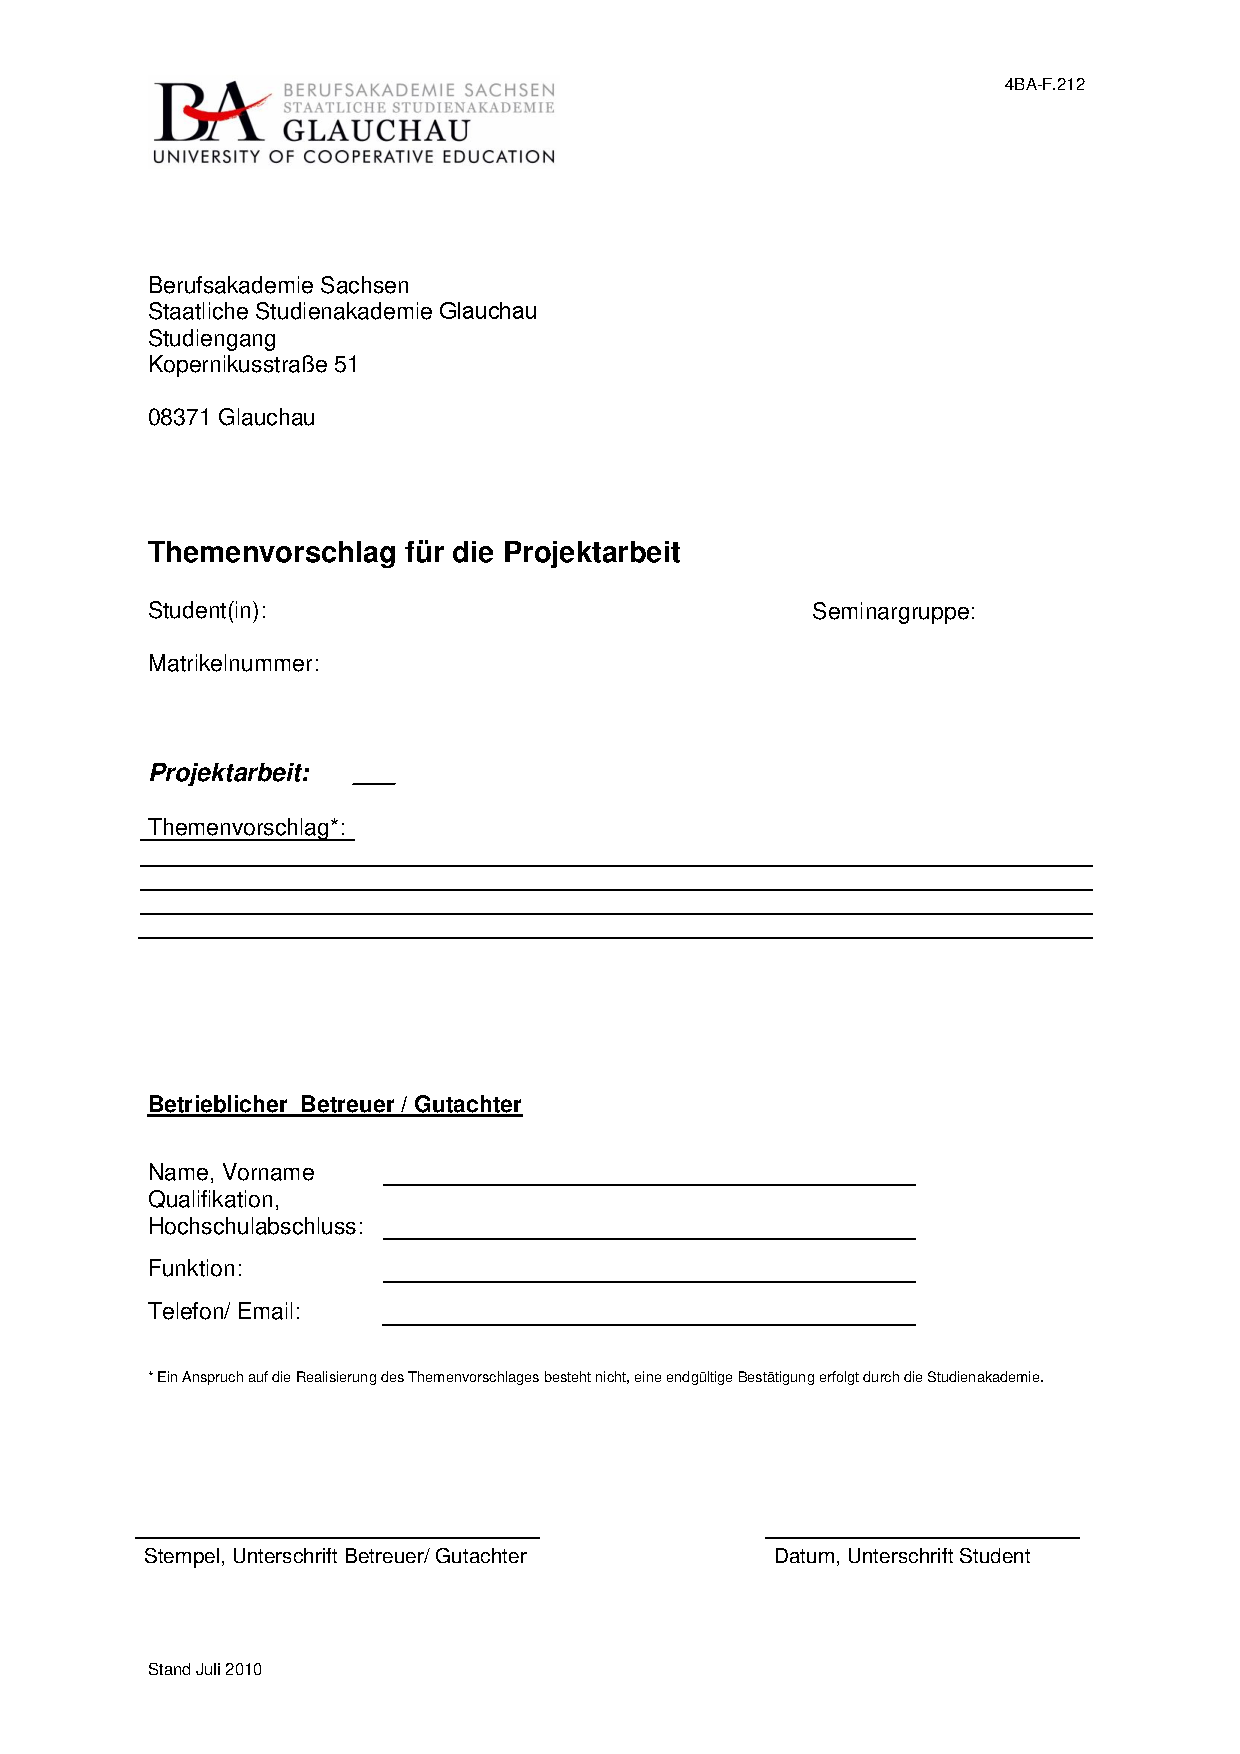
\includegraphics[scale=0.8]{Anhang/4BA-F.212_Themenvorschlag_für_die_Projektarbeit_ausfüllbar.pdf}
%TODO skalierung
\clearpage

\chapter{Themenvorschlag für die Bachelorthesis/Diplomarbeit}
\label{anhang-themenvorschlag-bt-dipl}
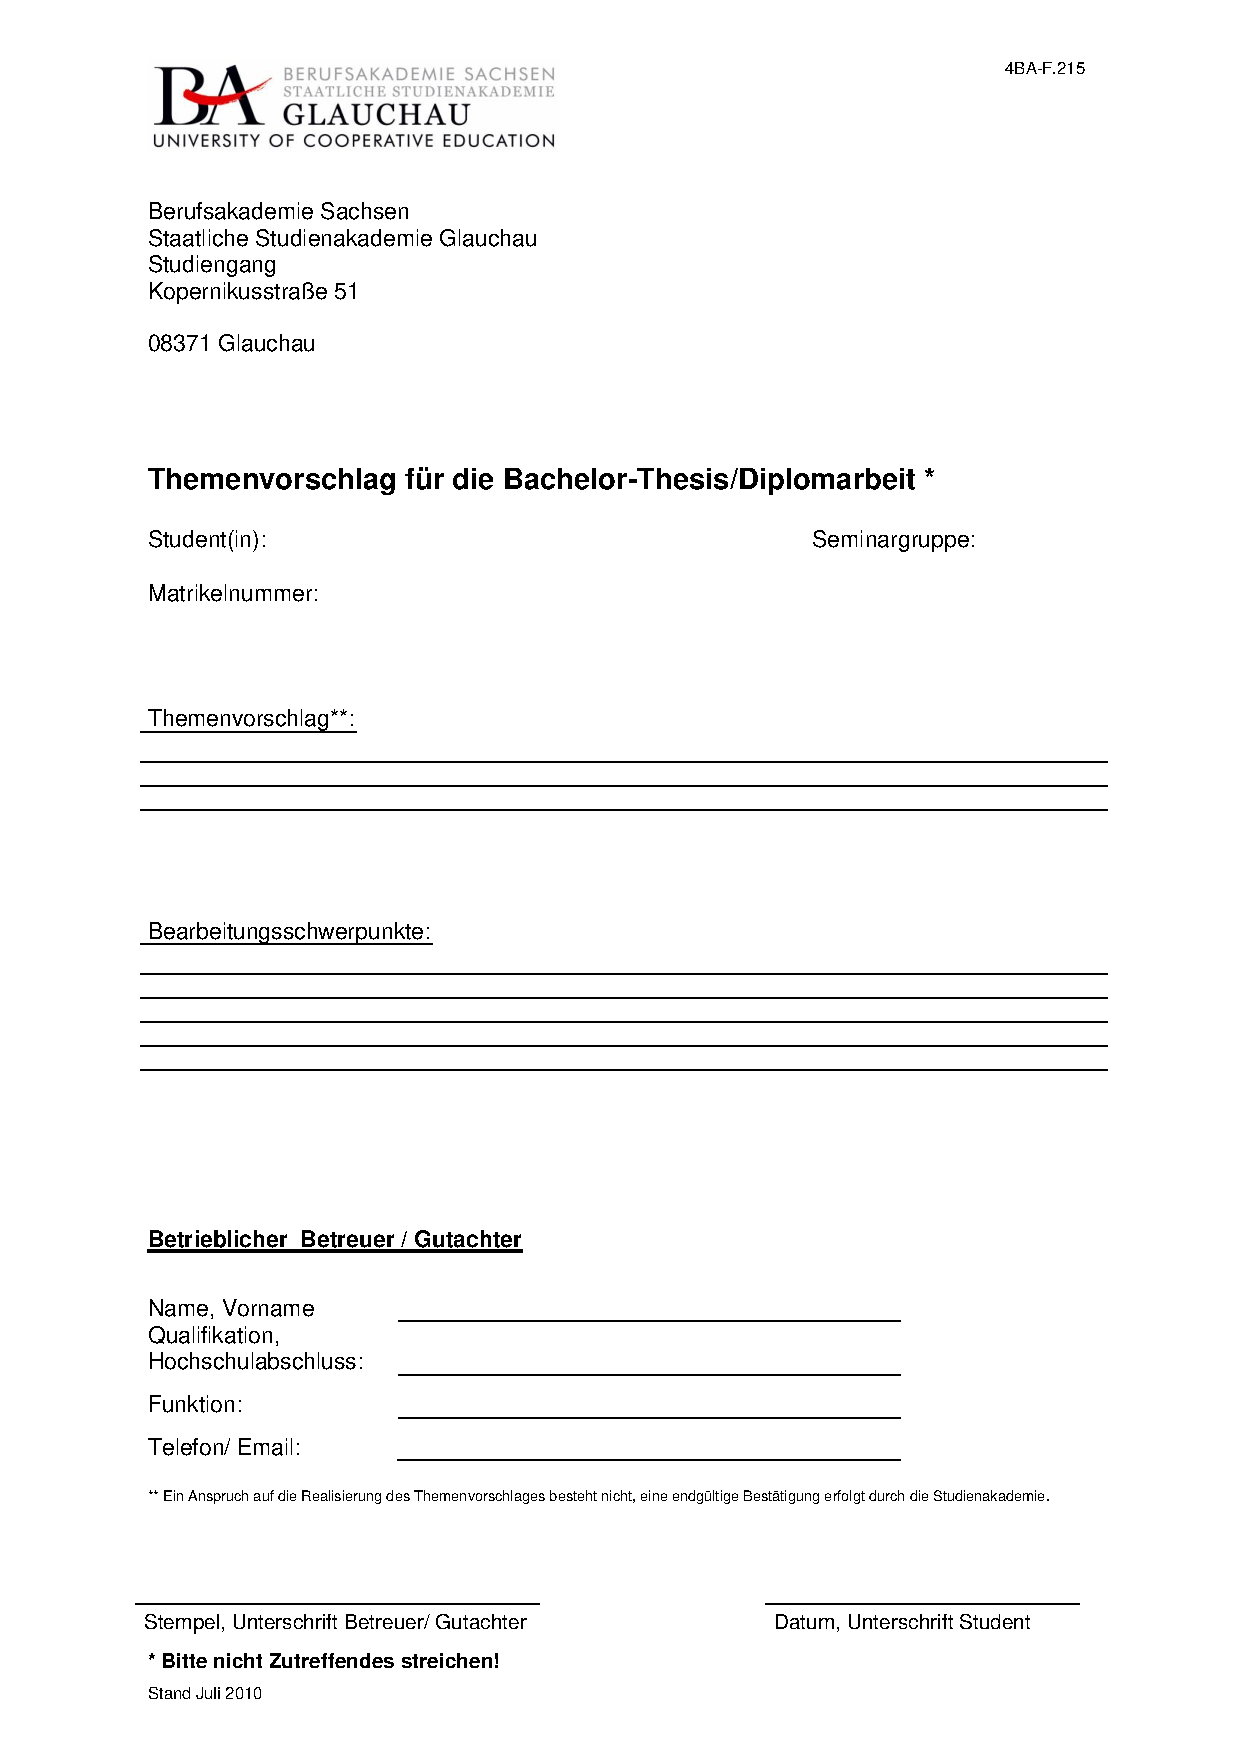
\includegraphics[scale=0.8]{Anhang/4BA-F.215_Themenvorschlag_für_die_Bachelor-Thesis_ausfüllbar.pdf}
%TODO skalierung
\clearpage
\hbadness=10000

%  Eidesstattliche Erklärung
%! Dies ist eine zur Nutzung mit LaTeX angepasste Version der in Anhang 6 der Hinweise zur Anfertigung
%! wissenschaftlicher Arbeiten an der Staatlichen Studienakademie Glauchau vorgegebenen Zustimmung
%! zur Plagiatsprüfung für Praxisbelege.
\cleardoublepage
\chapter{Ehrenwörtliche Erklärung}
    \vspace*{1cm}
    \begin{center}
        \huge\textbf{Ehrenwörtliche Erklärung}\\
    \end{center}
    \vspace*{1cm}
    \normalsize
    Ich erkläre hiermit ehrenwörtlich,

    \begin{enumerate}
        \vspace{1cm}
        \item dass ich \ifthenelse{\isundefined{\jahr}}{meinen Praxisbeleg}{meine Bachelorthesis} mit dem Thema:\\

        \textbf{\titel }\\

        ohne fremde Hilfe angefertigt habe,
        \item dass ich die Übernahme wörtlicher Zitate aus der Literatur sowie die\\
        Verwendung der Gedanken anderer Autoren an den entsprechenden\\
        Stellen innerhalb der Arbeit gekennzeichnet habe und
        \item dass ich \ifthenelse{\isundefined{\jahr}}{meinen Praxisbeleg}{meine Bachelorthesis} bei keiner anderen Prüfung vorgelegt habe.\\[1,5cm]
    \end{enumerate}
    Ich bin mir bewusst, dass eine falsche Erklärung rechtliche Folgen haben wird.\\[1,5cm]

    Glauchau, \abgabedatum \newline\noindent\rule{0.35\columnwidth}{0.4pt}\hspace{0.05\columnwidth}\rule{0.6\columnwidth}{0.4pt}\\
    Ort, Datum\hspace{0.27\columnwidth}Unterschrift

    \newpage
\chapter{Zustimmung Plagiatsprüfung}

    \vspace*{2mm}

    \begin{minipage}{0.5\columnwidth}
        \includesvg[width=\columnwidth]{vorlage/bilder/ba-gc-logo}
        % Alternativ mit PNG Logo, falls Inkscape nicht installiert werden, bzw. nicht der PATH-Variable hinzugefügt werden soll.
        %! Die SVG-Version sieht im Druck deutlich besser aus.
        %
\includegraphics[width=\columnwidth]{vorlage/bilder/ba-gc-logo}
    \end{minipage}
    \begin{minipage}{0.45\columnwidth}
        \begin{flushright}
            {\small nach 4BA-F.219\\}
        \end{flushright}
    \end{minipage}
    \vspace*{2mm}

    \begin{center}
        \textbf{\huge{Erklärung zur Prüfung wissenschaftlicher Arbeiten}}
    \end{center}

    Die Bewertung wissenschaftlicher Arbeiten erfordert die Prüfung auf Plagiate. Die hierzu von der Staatlichen Studienakademie Glauchau eingesetzte Prüfungskommission nutzt sowohl eigene Software als auch diesbezügliche Leistungen von Drittanbietern. Dies erfolgt gemäß \href{https://www.revosax.sachsen.de/vorschrift/1672-Saechsisches-Datenschutzgesetz#p7}{§ 7 des Gesetzes zum Schutz der informationellen Selbstbestimmung im Freistaat Sachsen (Sächsisches Datenschutzgesetz - SächsDSG)} vom 25. August 2003 (Rechtsbereinigt mit Stand vom 31. Juli 2011) im Sinne einer Datenverarbeitung im Auftrag.

    Der Studierende bevollmächtigt die Mitglieder der Prüfungskommission hiermit zur Inanspruchnahme o. g. Dienste. In begründeten Ausnahmefällen kann der Datenschutzbeauftragte der Berufsakademie Sachsen sowohl vom Verfasser der wissenschaftlichen Arbeit als auch von der Prüfungskommission in den Entscheidungsprozess einbezogen werden.

    \arrayrulewidth=0.5pt
    \begin{table}[H]
        \centering
        \begin{tabularx}{\columnwidth}{|p{3.2cm}|X|}
            \hline
            Name:             & \autoreins\\
            \hline
            Matrikelnummer:   & \matnumeins\\
            \hline
            Studiengang:      & \studiengang\\
            \hline
            Titel der Arbeit: & \titel\\
            \hline
            Datum:            & \abgabedatum\\
            \hline
            Unterschrift:     & \\
                              & \\
            \hline
        \end{tabularx}
    \end{table}

    \vfill

\clearpage

\input{vorlage/Freigabeerklärung_Bachelorthesis}
\clearpage

\chapter{Beispiel/Muster Abstract}
\label{anhang-abstract}
%TODO
Abstract einbauen
\hbadness=1000
%!##########################################

\end{document}
